\documentclass[times, utf8, zavrsni]{fer}
\usepackage{booktabs}


\usepackage[croatian]{babel} 
\usepackage{amssymb}
\usepackage{amsmath}
\usepackage{txfonts}
\usepackage{mathdots}
\usepackage{titlesec}
\usepackage{array}
\usepackage{lastpage}
\usepackage{etoolbox}
\usepackage{tabularray}
\usepackage{color, colortbl}
\usepackage{adjustbox}
\usepackage{geometry}
\usepackage[classicReIm]{kpfonts}
\usepackage{hyperref}
\usepackage{fancyhdr}
\usepackage[T1]{fontenc}     % default is 'OT1'
\usepackage[utf8]{inputenc}
\usepackage{graphicx}

\usepackage{float}
\usepackage{setspace}
\restylefloat{table}


%boja za privatni i udaljeni kljuc u tablicama
\definecolor{LightBlue}{rgb}{0.9,0.9,1}
\definecolor{LightGreen}{rgb}{0.9,1,0.9}

%Promjena teksta za dugačke tablice
\DefTblrTemplate{contfoot-text}{normal}{Nastavljeno na idućoj stranici}
\SetTblrTemplate{contfoot-text}{normal}
\DefTblrTemplate{conthead-text}{normal}{(Nastavljeno)}
\SetTblrTemplate{conthead-text}{normal}
\DefTblrTemplate{middlehead,lasthead}{normal}{Nastavljeno od prethodne stranice}
\SetTblrTemplate{middlehead,lasthead}{normal}


%Programski kod
\usepackage{courier} %% Sets font for listing as Courier.
\usepackage{listings, xcolor}
\lstset{
tabsize = 4, %% set tab space width
showstringspaces = false, %% prevent space marking in strings, string is defined as the text that is generally printed directly to the console
numbers = left, %% display line numbers on the left
commentstyle = \color{green}, %% set comment color
keywordstyle = \color{blue}, %% set keyword color
stringstyle = \color{red}, %% set string color
rulecolor = \color{black}, %% set frame color to avoid being affected by text color
basicstyle = \scriptsize \ttfamily , %% set listing font and size
breaklines = true, %% enable line breaking
numberstyle = \tiny,
}




\begin{document}

% TODO: Navedite broj rada.
\thesisnumber{663}

% TODO: Navedite naslov rada.
\title{Mobilna igra za vježbanje matematike}

% TODO: Navedite vaše ime i prezime.
\author{Denis Pipalović}

\maketitle

% Ispis stranice s napomenom o umetanju izvornika rada. Uklonite naredbu \izvornik ako želite izbaciti tu stranicu.
\izvornik

% Dodavanje zahvale ili prazne stranice. Ako ne želite dodati zahvalu, naredbu ostavite radi prazne stranice.
\zahvala{}

\tableofcontents

\chapter{Uvod}
	Matematika, osim što je predmet koji se predaje u svim razredima osnovnih i srednjih škola, također je i znanost iz područja prirodnih znanosti.
Značaj matematike vidljiv je ne samo u drugim poljima područja prirodnih znanosti, već i u svim drugim područjima, posebice u području tehničkih znanosti.
Ne poznavanje osnova matematike negativno se odražava na učenikove školske uspjehe kroz cijelo školovanje. Jedan od problema svakako je problem pristupa nastavnika
 u učenju matematike, odnosno manjak povlačenja paralela sa stvarnim svijetom i pokazivanja primjena matematike; ovakav pristup demotivira učenika u vježbanju matematike
i savladavanju čak i osnovnih računskih operacija. Jednom izgubljenu motivaciju za neko područje teško je vratiti nazad.

Primjenom gamifikacije u edukaciji učenicima bi se razne teme i ishodi učenja mogle prezentirati kroz zanimljive načine, samim time i povećati zainteresiranost za nekom temom 
ili predmetom. S obzirom na to da djeca u novije doba koriste pametne uređaje sve više i više, gamifikacija jedan od način kroz koji bi to vrijeme na mobitelu moglo biti potrošeno
 u edukativne svrhe; kroz zabavu!

S obzirom na navedeno, tema ovog rada je napraviti mobilnu igru za vježbanje matematike u nižim razredima osnovne škole koja će kroz zanimljiv i interaktivan način pružati  ugodnije iskustvo
vježbanja matematičkih zadataka. Igra je zamišljena kao tzv. „endless runner“ u kojoj igrač skuplja padajuće objekte ovisno o trenutnom zadatku (npr. samo parne brojeve, brojeve veće od zadanog,
brojeve djeljive s određenim brojem, samo kvadrate i slično) i sakuplja bodove. Kako igra ne bi postala monotona kroz kratko vrijeme igranja cilj je napraviti da igra postaje progresivno sve teža
i teža, no do te mjere da se ne postigne negativan efekt u drugom ekstremu; igra ne smije postati niti previše teška jer bi samim time postala i demotivirajuća! Stoga je cilj da se težina igre
dinamički prilagođava mogućnostima učenika. Osim same mobilne igre, potrebno je izgraditi i jednostavno web sučelje za učitelja kako bi mogao postavljati tipove zadataka koji prate temu onoga što
se trenutno predaje na nastavi. Kroz navedeno web sučelje nastavniku će se pružati i mogućnost pregleda rezultata pojedinog učenika te uvid u detalje igre kao što je tip zadatak na kojem je učenik 
griješio, ukupno vrijeme igranja i slično. Kako bi igra bila dostupna svima koji ju požele igrati, odnosno kako igra ne bi ovisila o postavkama učitelja, postojati će i zadane postavke koje će se moći
 prilagođavati kroz postavke same igre. 



\chapter{Cilj projekta}
Cilj projekta je izrada mobilne igre za vježbanje matematike popraćene web stranicom koja služi za zadavanje zadataka i pregled rezultata igre. Cilj mobilne igre napraviti je vježbu matematike zanimljiviju učenicima, 
dok je cilj web stranice učiteljima olakšati zadavanje zadataka, praćenje i pohranu rezultata učenika na jednostavniji način.

	\section{Mobilna igra}
	Mobilna igra većinski je dio projekta. Kroz ovu igru učenici nižih razreda na zanimljiviji način mogu vježbati određeno gradivo matematike. Igra osim što se može igrati s predefiniram postavkama zadataka također omogućava uređivanje istih
	te preuzimanje postavki koje su napravljene preko web sučelja za učitelja. Ukoliko učenik igra igru sa preuzetim postavkama napravljenim preko web sučelja, podaci o njegovoj igri bit će dostavljeni učitelju po završetku igre.
	Iz glavnog menija igre možemo pristupiti glavnom ekranu igre i postavkama.
		
		\subsection{Glavni ekran igre}
		Na glavnom ekranu igre nalazi se sav takoreći učenicima zanimljiv sadržaj, odnosno mjesto gdje se sama igra i igra. Igra je "endless runner" i tematski je zamišljena kao put iz središta zemlje ka dubokom svemiru, odnosno to je ono što pokazuje
		pozadina koja putuje prema dolje, što stvara efekt putovanja objekta koji se upravlja prema gore. Objekt koji je upravljan moguće je pomicati lijevo-desno i tako skupljati padajuće objekte koje je potrebno skupiti ovisno o trenutnom zadatku,
		odnosno izbjegavati one koji krše pravila trenutnog zadatka. Padajući objekti konstanto se stvaraju i njihov sadržaj ovisi o tome koji je trenutni zadatak ili koja je trenutna težina igre. Odnosno svaki zadatak osim što ima svoj opis ima i određene
		parametre, tako bi recimo zadak "skupljaj brojeve veće ili jednake 18", osim navedenog opisa, relativnog broja 18 imao i definirane parametre kao što je minimalna i maksimalna granica iz kojeg seta se brojevi mogu dodjeliti; nadalje, pri većoj 
		težini igre se na padajućem objektu možda neće prikazati broj direktno, već u obliku matematičke operacije, npr. "29 - 12".
		\begin{figure}[H]
			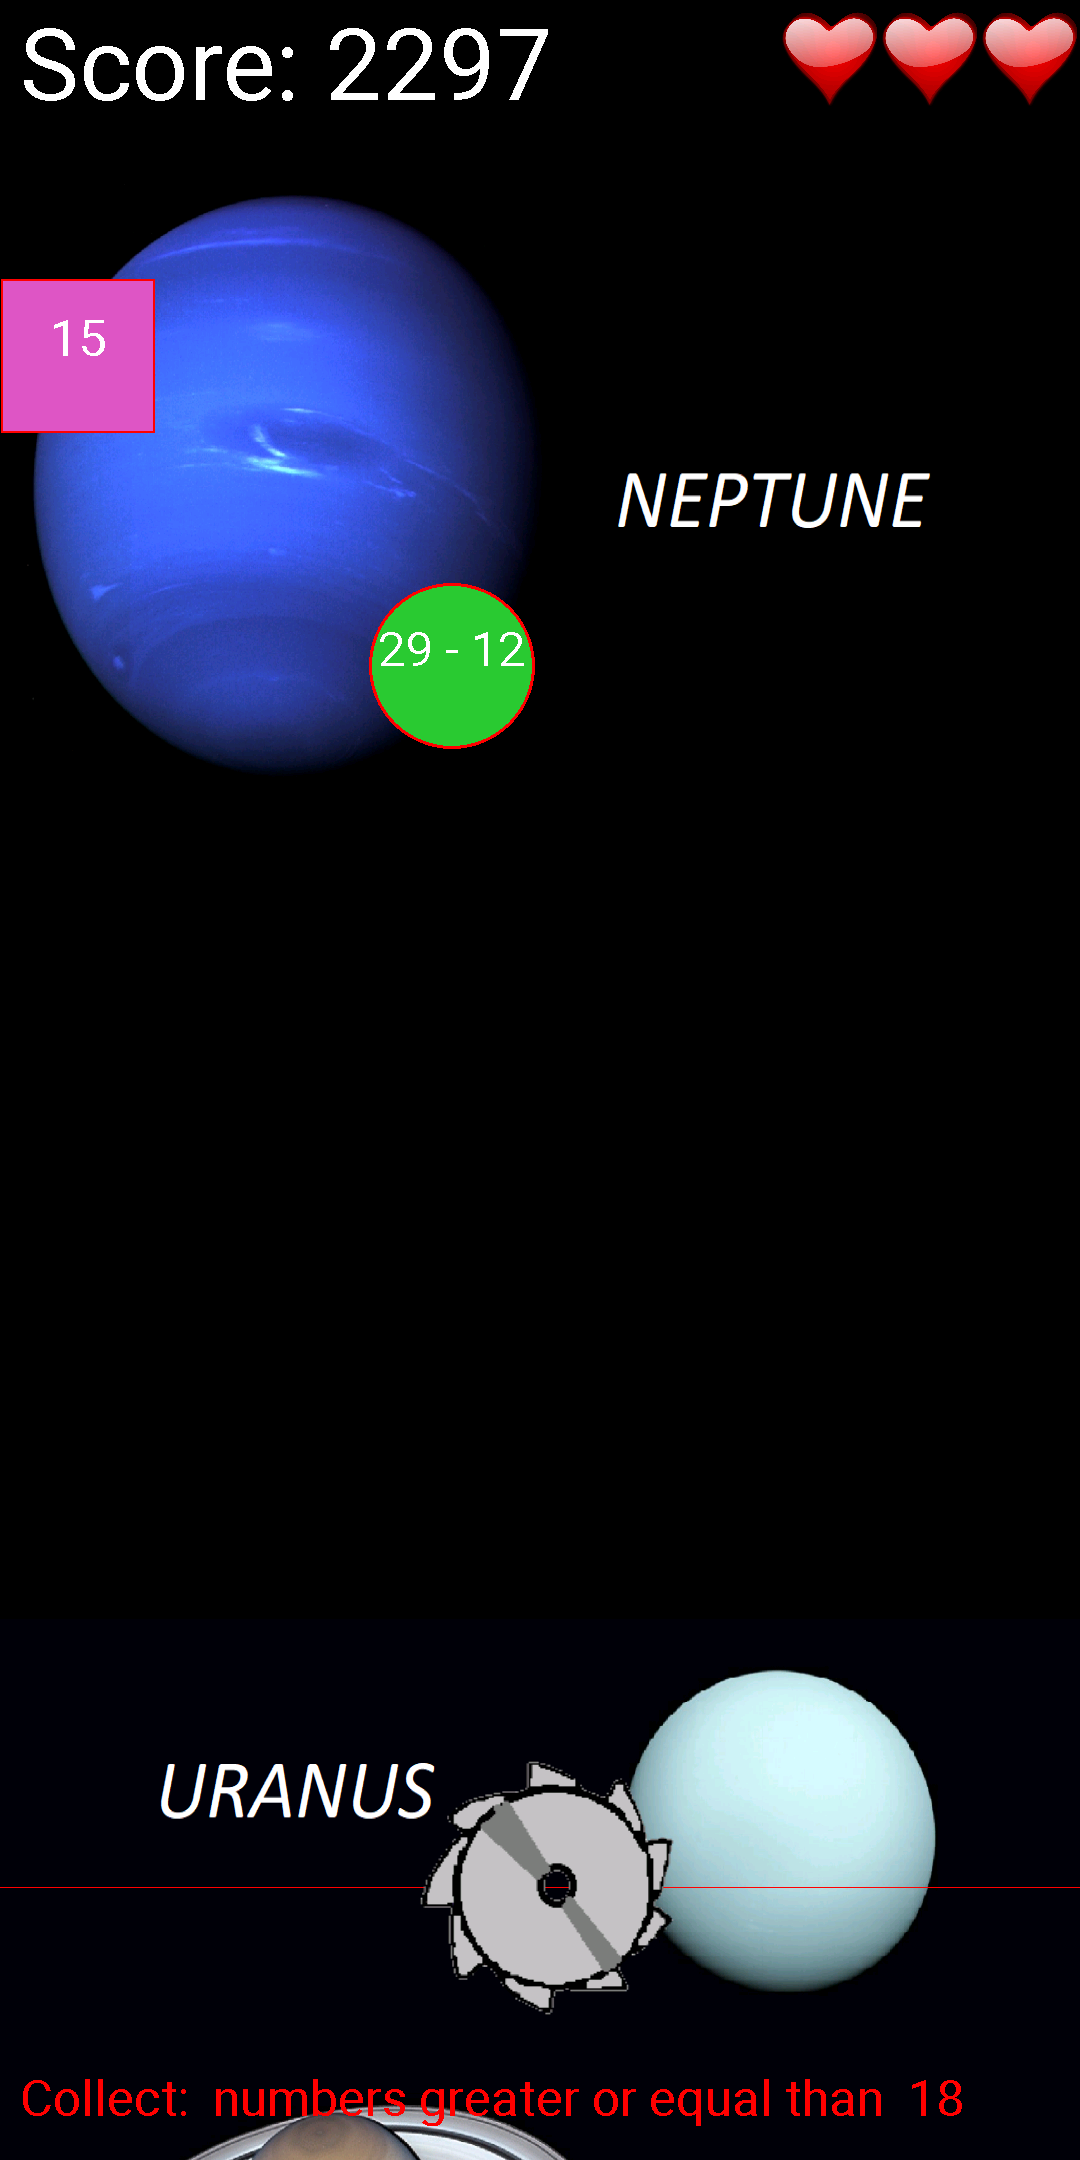
\includegraphics[scale = 0.225]{"slike/igra.png"} 
			\centering
			\caption{Ideja igre}
			\label{fig:idejaigre}
		\end{figure}
		
		Igranjem igre i sakupljanjem objekata koji odgovaraju trenutačnom zadatku učenici skupljaju bodove; te je cilj po završetku igre imati što veći broj bodova. Završetak igre odgovara gubitku tri života.
		Bodovanje na primjeru  za zadatak "skupljaj parne brojeve" :
		\begin{itemize}
				\item  {Igrač je pokupio paran broj : +100 bodova}
				\item  {Igrač NIJE pokupio paran broj: -100 bodova}
				\item  {Igrač je pokupio neparan broj: Gubitak života}
		\end{itemize}
		
		S obzirom da se može dogoditi situacija u kojoj se preklapaju dva objekta, odnosno situacija u kojoj se preklapaju objekt koji se ne smije pokupiti i objek koji se mora pokupiti (u ovom slučaju parni i neparni broj); kako se igrač ne bi osjećao
		zakinutim nakon gubitka 100 bodova zbog objekta kojeg je morao propustiti kako ne bi izgubio jedan život, igrač je za svakih 10 osvježavanja ekrana nagrađen sa jednim bodom. U konačnici ispada da igrač smije propustiti jedan objekt svakih 15 do 20 sekundi
		kako bi se poništili bonus bodovi sa izgubljenim bodovima za ne skupljanje odgovarajućeg objekta. Preklapanje dva objekta se ne događa toliko često stoga igrač samim trajenjem igre skuplja dodatne bodove.
		\newline
		Trenutačni broj bodova prikazan je na vrhu zaslona sa lijeve strane, dok je na desnoj strani prikazan broj života koji odgovara broju sličica srca. Na donjem dijelu ekrana moguće je vidjeti trenutačni zadatak.
		Svaki zadatak traje od prilike pola minute, a promijena zadatka odvija se na način da prvo prestanu padati novi objekti. Kada više nema padajućih objekata na ekranu, slučajnim odabirom se bira sljedeći zadatak te se tekst novog zadatka
		pokazuje kako u donjem dijelu ekrana tako i na samoj sredini ekrana na nekoliko sekundi kako bi igrač bio u potpunosti svjestan promjene zadatka. 

		
		\subsection{Predefinirane postavke}
		Kako igra ne bi ovisila isključivo o postavkama koje zadaje učitelj, odnosno kako bi se mogla igrati neposredno nakon instalacije, osmišljene su predefinirane postavke koje sadrže zadatke prilagođene ponajviše prvom razredu osnovne škole.
		Neki od predefiniranih zadataka su: 
			\begin{itemize}
				\item  {Skupljaj parne brojeve}
				\item  {Skupljaj neparne brojeve}
				\item  {Skupljaj brojeve veće od \textit{x}}
				\item  {Skupljaj brojeve manje od \textit{x}}
				\item  {Skupljaj brojeve veće ili jednake \textit{x} koji su parni }
				\item  {Skupljaj kvadrate}
				\item  {Skupljaj kružnice}
				\item {i slično}
			\end{itemize}
		Osim što igra omogućava ove i druge predefinirane postavke, također omogućava i njihovo uređivanje, odnosno njihovo uključivanje te isključivanje; kako bi si učenici samostalno mogli prilagoditi zadatke na koje žele staviti naglasak dok vježbaju.
		Svako uključivanje, odnosno isključivanje navedenog zadatka ostaje zapamćeno i koristi se pri pokretanju igre.
		
		\begin{figure}[H]
			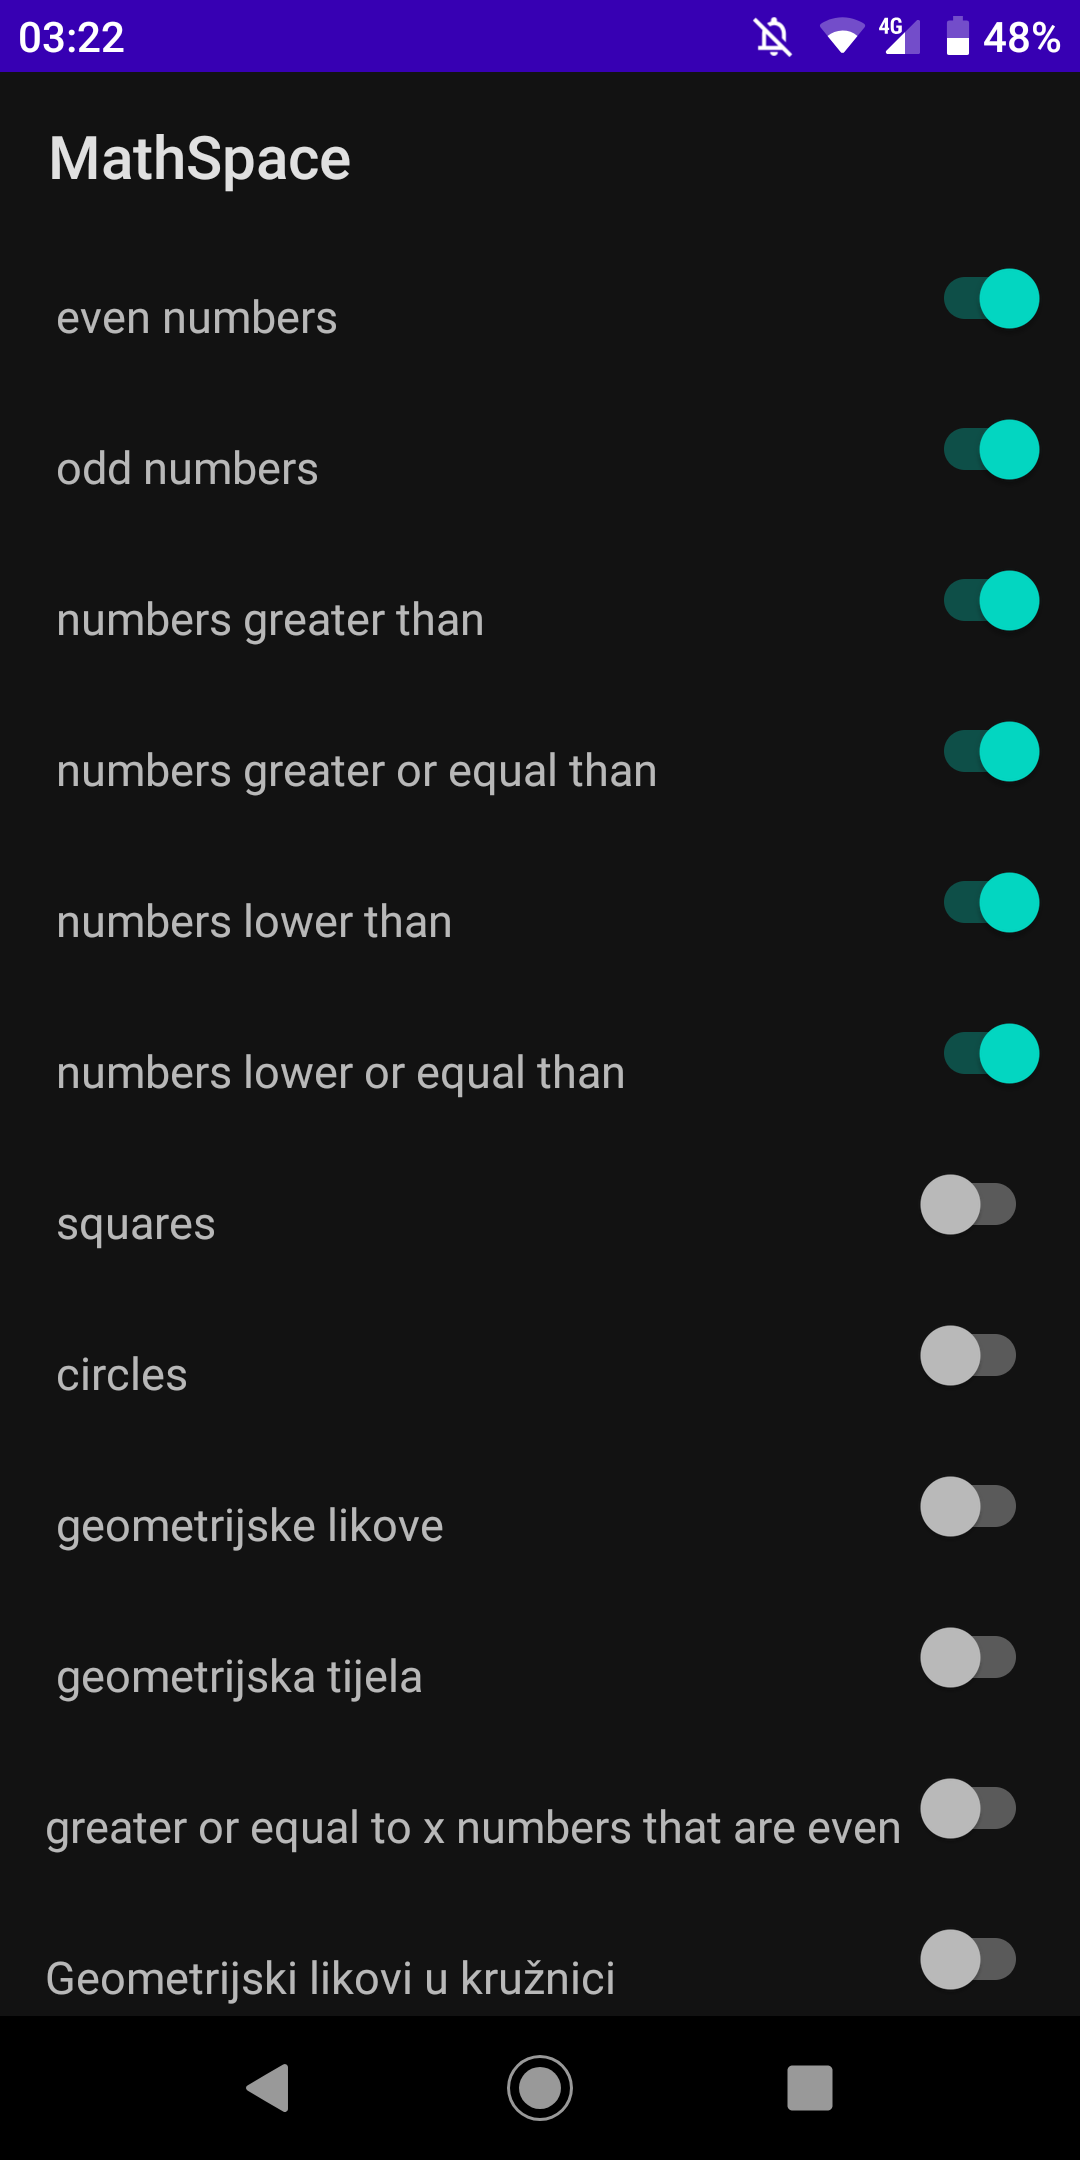
\includegraphics[scale = 0.1]{"slike/defaulttasks.png"} 
			\centering
			\caption{Ideja Uključivanje/isključivanje predefiniranih postavki}
			\label{fig:idejaigre}
		\end{figure}
		

		\subsection{Preuzete postavke}
		Osim predefiniranih postavki igra nudi mogućnost preuzimanja postakvi izrađenih preko web stranice. Kako bi igrač mogao preuzeti postavke prvo treba postaviti korisničko ime te nakon toga u za to previđeno polje upisati identifikator postavki
		koje želi preuzeti i za kraj pritisnuti tipku za preuzimanje postavki. 
	
		\begin{figure}[H]
			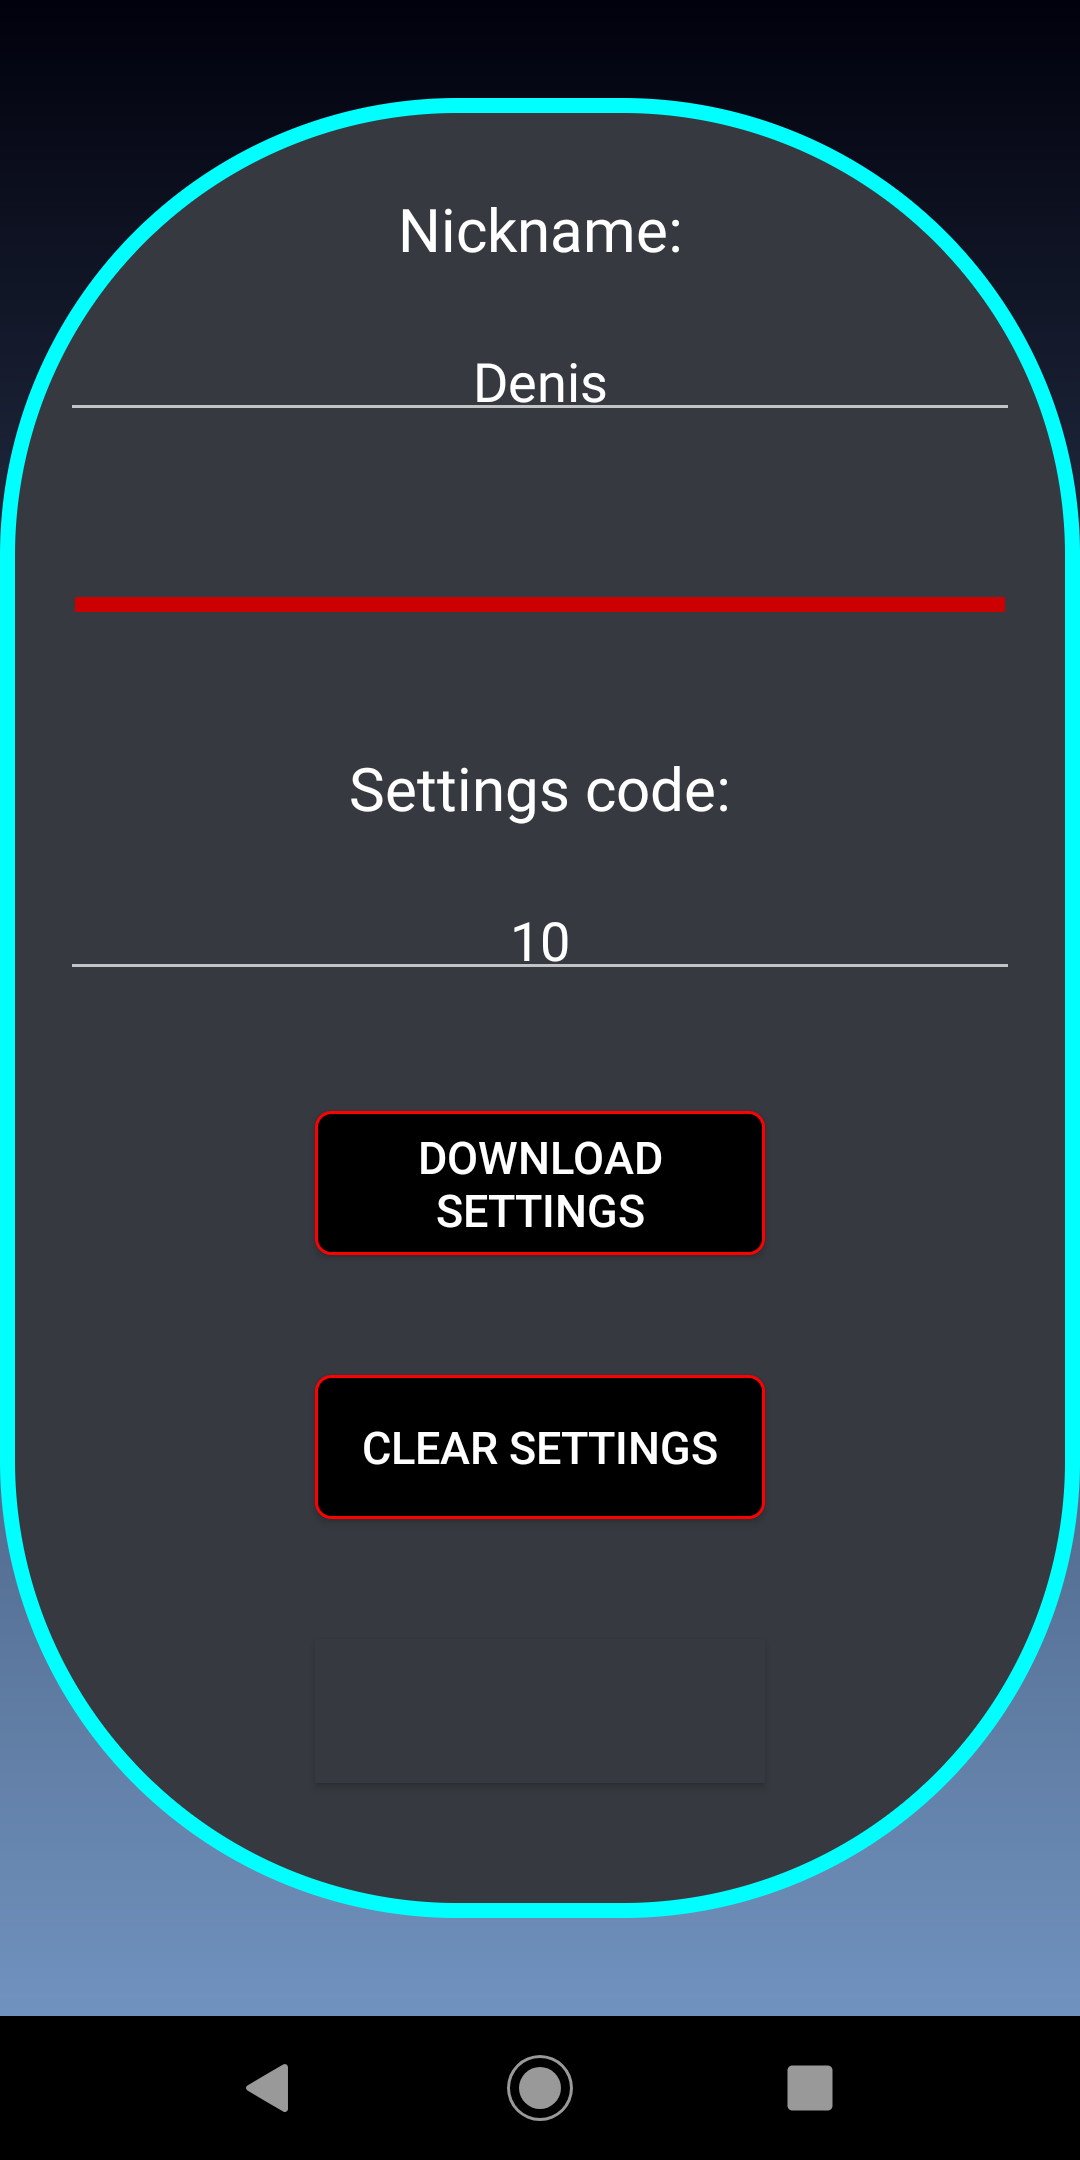
\includegraphics[scale = 0.2]{"slike/downloadsettings.png"} 
			\centering
			\caption{Preuzimanje postavki s interneta}
			\label{fig:preuzimanjepostavki}
		\end{figure}
		
		Jednom kad je igrač preuzeo postavke s interneta sada mu se na izbor u glavnom meniju postavki pruža mogućnost odabira koje postavke želi koristiti; one preuzete s interneta ili one predefinirane!
		
				\begin{figure}[!htb]
			\begin{minipage}{0.48\textwidth}
				\centering
				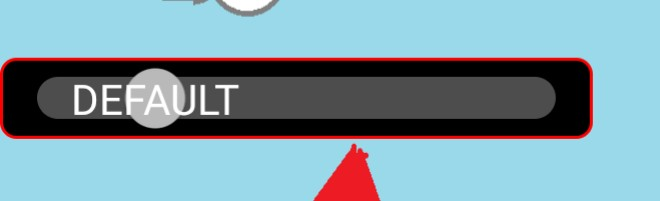
\includegraphics[scale=0.25]{"slike/usedefault.jpg"} 
				\caption{Odabir korištenja predefiniranih postavki}
				\label{fig:saw1}
			\end{minipage}\hfill
			\begin{minipage}{0.48\textwidth}
				\centering
				
\includegraphics[scale=0.25]{"slike/usedownloaded.jpg"} 
				\caption{Odabir korištenja preuzetih postavki}
				\label{fig:saw2}
			\end{minipage}
		\end{figure}
		
		

	\section{Web stranica}
	Web stranica drugi je dio projekta, ujedno i manji. Kroz ovu web stranicu učiteljima se na jednostavan način omogućava izrada zadataka, odnosno postavljanje pravila na osnovu kojih će se zadaci automatski generirati.
	Osim zadavanja zadataka stranica nudi i mogućnost pregleda rezultata pojedinih učenika i dodatne dalje svakog igranja. Za mogućnost izrade postavki, stoga i pregled rezultata igrara korisnik se mora prvo prijaviti u sustav, odnosno
	registrirati ukoliko nema korisnički račun.

	\subsection{Izrada postavki}
	Izrada postavki generalno je jednostavan i izravan (engl. \textit{straightforward}) proces. Nakon logiranja u sustav korisniku se nudi opcija "\textit{My Games}" na izbornoj traci. Odabirom ove stavke korisniku se prikazuju sve
	njegove postojeće grupe postavke igara i mogućnost izrada nove grupe postavki. 
	
		\begin{figure}[H]
			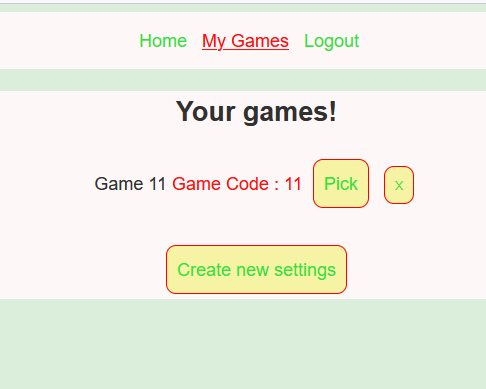
\includegraphics[scale = 0.7]{"slike/izradapostavki.png"} 
			\centering
			\caption{My Games}
			\label{fig:izradapostavki}
		\end{figure}
	
	Odabir postojeće grupe postavki moguće je učiniti pritiskom na gumb "\textit{Pick}" uz postavke koje želimo odabrati, odnosno ukloniti grupu postavki klikom na  gumb "\textit{X}". Izrada nove grupe postavki može se napraviti klikom na gumb
	 "\textit{Create new settings}". 
	 

	 Nakon odabira određene grupe postavki korisniku se nudi mogućnost pregleda do sad napravljenih postavki pa tako i dodavanja nove postavki u odabranu grupu. Kako bi korisnik dodao novu postavku u grupu postavki prvo se treba odlučiti koji 
	 tip postavke želi dodati. 
	 	\begin{figure}[H]
			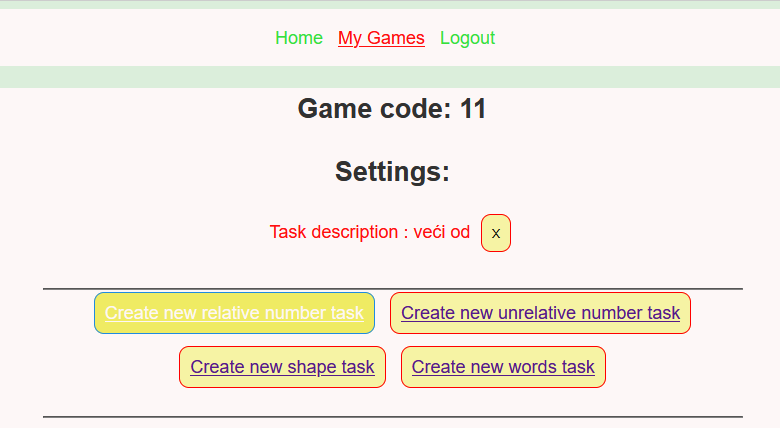
\includegraphics[scale = 0.7]{"slike/zadavanjepostavki.png"} 
			\centering
			\caption{Pregled i izrada postavki unutar neke grupe postavki}
			\label{fig:pregledpostavki}
		\end{figure}
	Na primjer, ukoliko korisnik želi zadati postavku koja od igrača mobilne igre traži da skuplja brojeve djeljive sa tri, potrebno je pritisnuti \textit{Create new relative number task} nakon čega se prikazuje novi ekran koji to omogućava.
	\begin{figure}[H]
		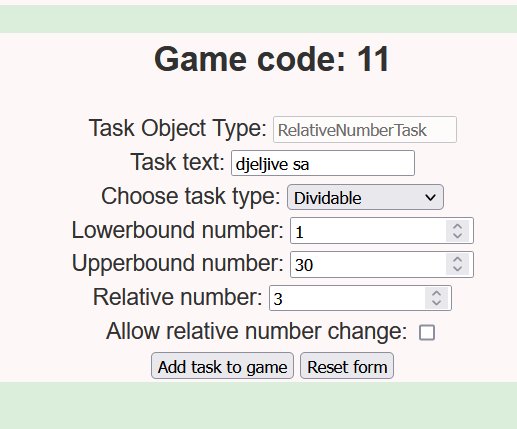
\includegraphics[scale = 0.9]{"slike/zadavanjekonkretnepostavke.png"} 
		\centering
		\caption{Izrada konkretne postavke}
		\label{fig:izradapostavkedjeljenje}
	\end{figure}
		
		Web stranica od korisnika traži unos teksta koji će opisivati zadatak, odabir tipa zadatka, donju i gornju granicu iz koje će se generirati brojevi na padajućim objektima, relativan broj odnosno, s obzirom da želimo zadati da je zadatak
		skupljati brojeve djeljive sa 3 - to je u ovom slučaju broj 3! Za kraj nudi se opcija promjene relativnog broja po završetku zadatka (novi broj slučajno bi se odredio iz skupa [lowerbound number, upperbound number]), što u ovom slučaju ne bismo
		htjeli. Ova opcija najviše je pogodna za zadatke koji od korisnika traže da skupljaju brojeve veće/manje od relativnog broja. Za završetak izrade postavke potrebno je odabrati \textit{Add task to game}.
	
	\subsection{Pregled rezultata}
	Nakon igranja igre na mobilnoj igri s preuzetim postavkama rezultati igre i njeni detalji postaju vidljivi korisniku web stranice koji je napravio korištene postavke. 
	Površni pregled koji prikazuje zapise o igrama prikazuje samo ime igrača, vrijeme prihvata podataka i konačni rezultat.
	\begin{figure}[H]
		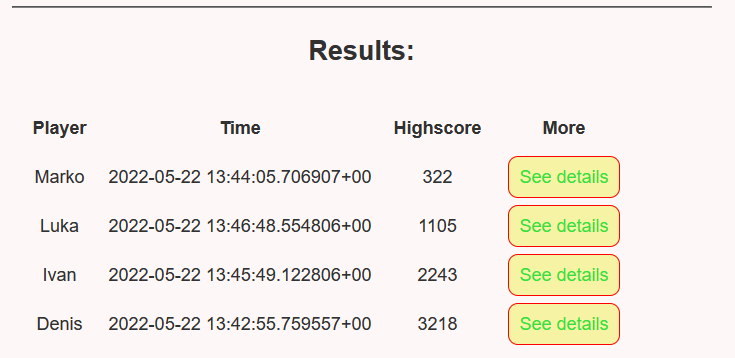
\includegraphics[scale = 0.9]{"slike/pregledsvihrezultata.png"} 
		\centering
		\caption{Pregled svih rezultata}
		\label{fig:pregledsvihrezultata}
	\end{figure}
	
	Odabirom gumba \textit{See details} korisniku web stranice pruža se mogućnost pregleda više detalja, odnosno mogućnost pregleda detalja cijelog tijek igre. Konkretnije omogućen je uvid u svaki značajniji događaj i njegovo vrijeme.
	Značajniji događaji su:
		\begin{itemize}
				\item  {Promjena zadatka - prikazano crnom bojom}
				\item  {Skupljen odgovarajući padajući objekt (+100 bodova) - prikazano zelenom bojom}
				\item  {Nije skupljen odgovarajući padajući objekt (-100 bodova) - prikazano naračastom bojom}
				\item  {Skupljen neodgovarajući objekt (izgubljen život) - prikazano crvenom bojom}
		\end{itemize}
	Radi jednostavnosti pregleda događaja igre, određeni događaji su istaknuti određenom bojom.
	
	\begin{figure}[H]
		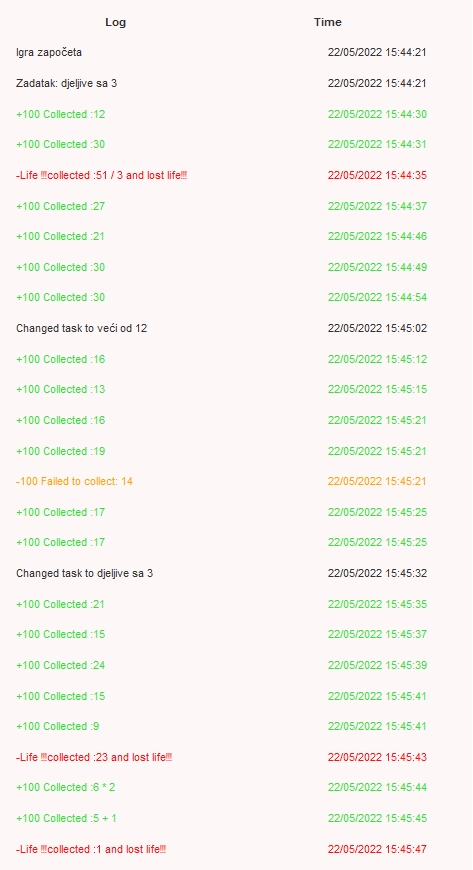
\includegraphics[scale = 0.9]{"slike/detaljanpregledrezultata.png"} 
		\centering
		\caption{Detaljan pregled jedne igre}
		\label{fig:pregledjedneigre}
	\end{figure}
	

\chapter{Usporedba sa sličnim igrama}
Postoje mnogobrojne Android igre dostupne na Google Play marketu koje kao su prikazane kao igre koje služe u edukativne svrhe, odnosno specifično kao igre za vježbanje matematike.  U nastavku je usporedba igre koja je tema ovog rada sa naizgled 
sličnim postojećim igrama; uz to valja i napomenuti da je po slobonoj procijeni više od 90% matematičkih igara bazirano na tipu kviza sa 4 ponuđena odgovora. Prednost igre koja je tema ovog rada nad navedenim igrama je mogućnost pregleda tijeka događaja.
	
	\section{Toon Math Runner} 
	"\textit{Toon Math Runner}" (u nastavku TMR) je vizualno lijepa 2.5D mobilna igra za vježbanje matematike. Ova igra nudi opciju otključavanja raznih karaktera u zamijenu za novčiće koje igrač može skupljati. Igrač upravlja karakterom
		na način da upravljenog karaktera može pozicionirati u jednoj od tri linije, osim toga nudi se mogućnost skakanja i saginjanja. Ova igrica uvelike podsjeća na popularnu igricu "\textit{Subway Surfers}" kako po načinu igranja, tako i vizualno.
	
		\begin{figure}[!htb]
			\begin{minipage}{0.48\textwidth}
				\centering
				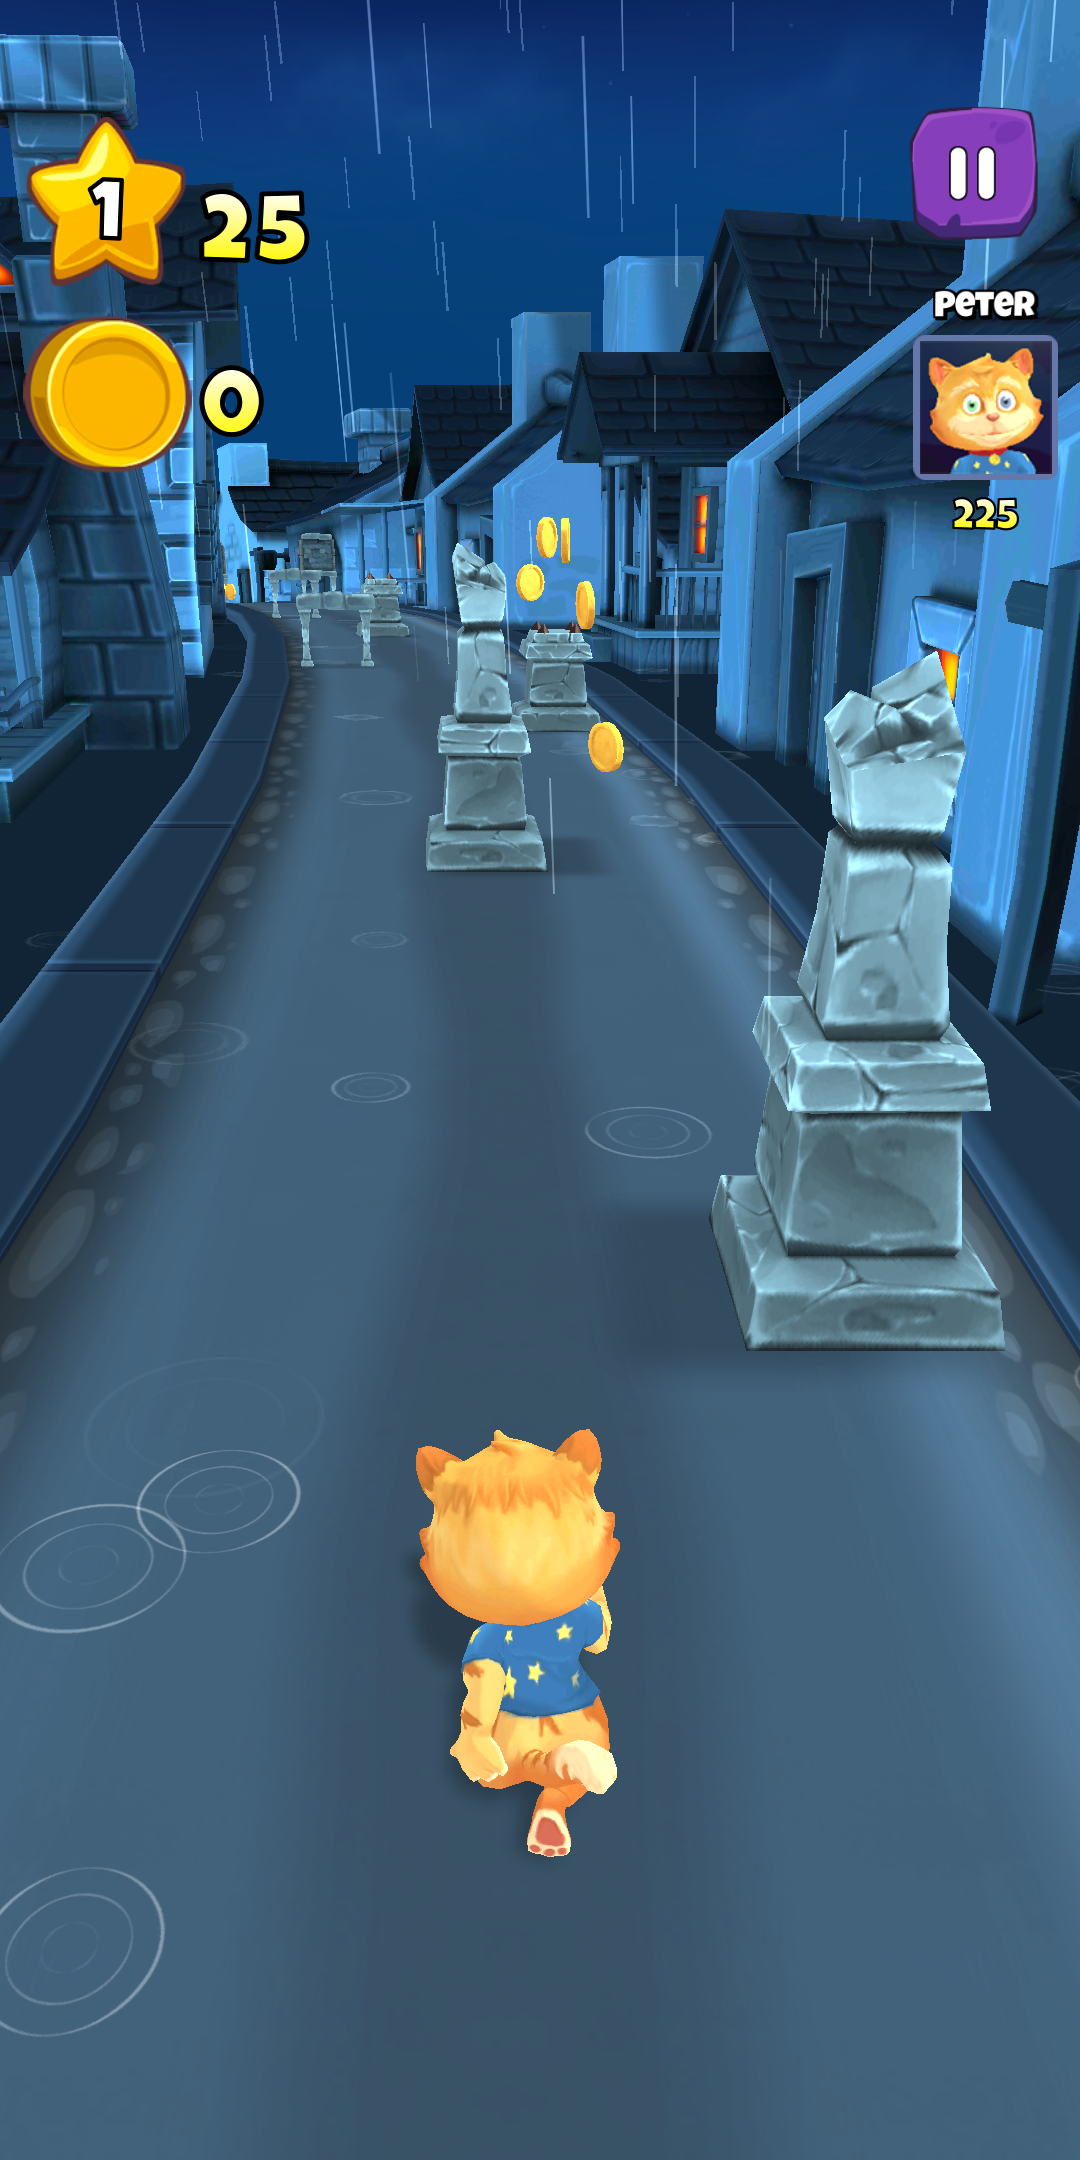
\includegraphics[scale=0.15]{"slike/igre/toonmath1.png"} 
				\caption{Većina igre - skupljanje novčića}
				\label{fig:skupljewnjenovcica}
			\end{minipage}\hfill
			\begin{minipage}{0.48\textwidth}
				\centering
				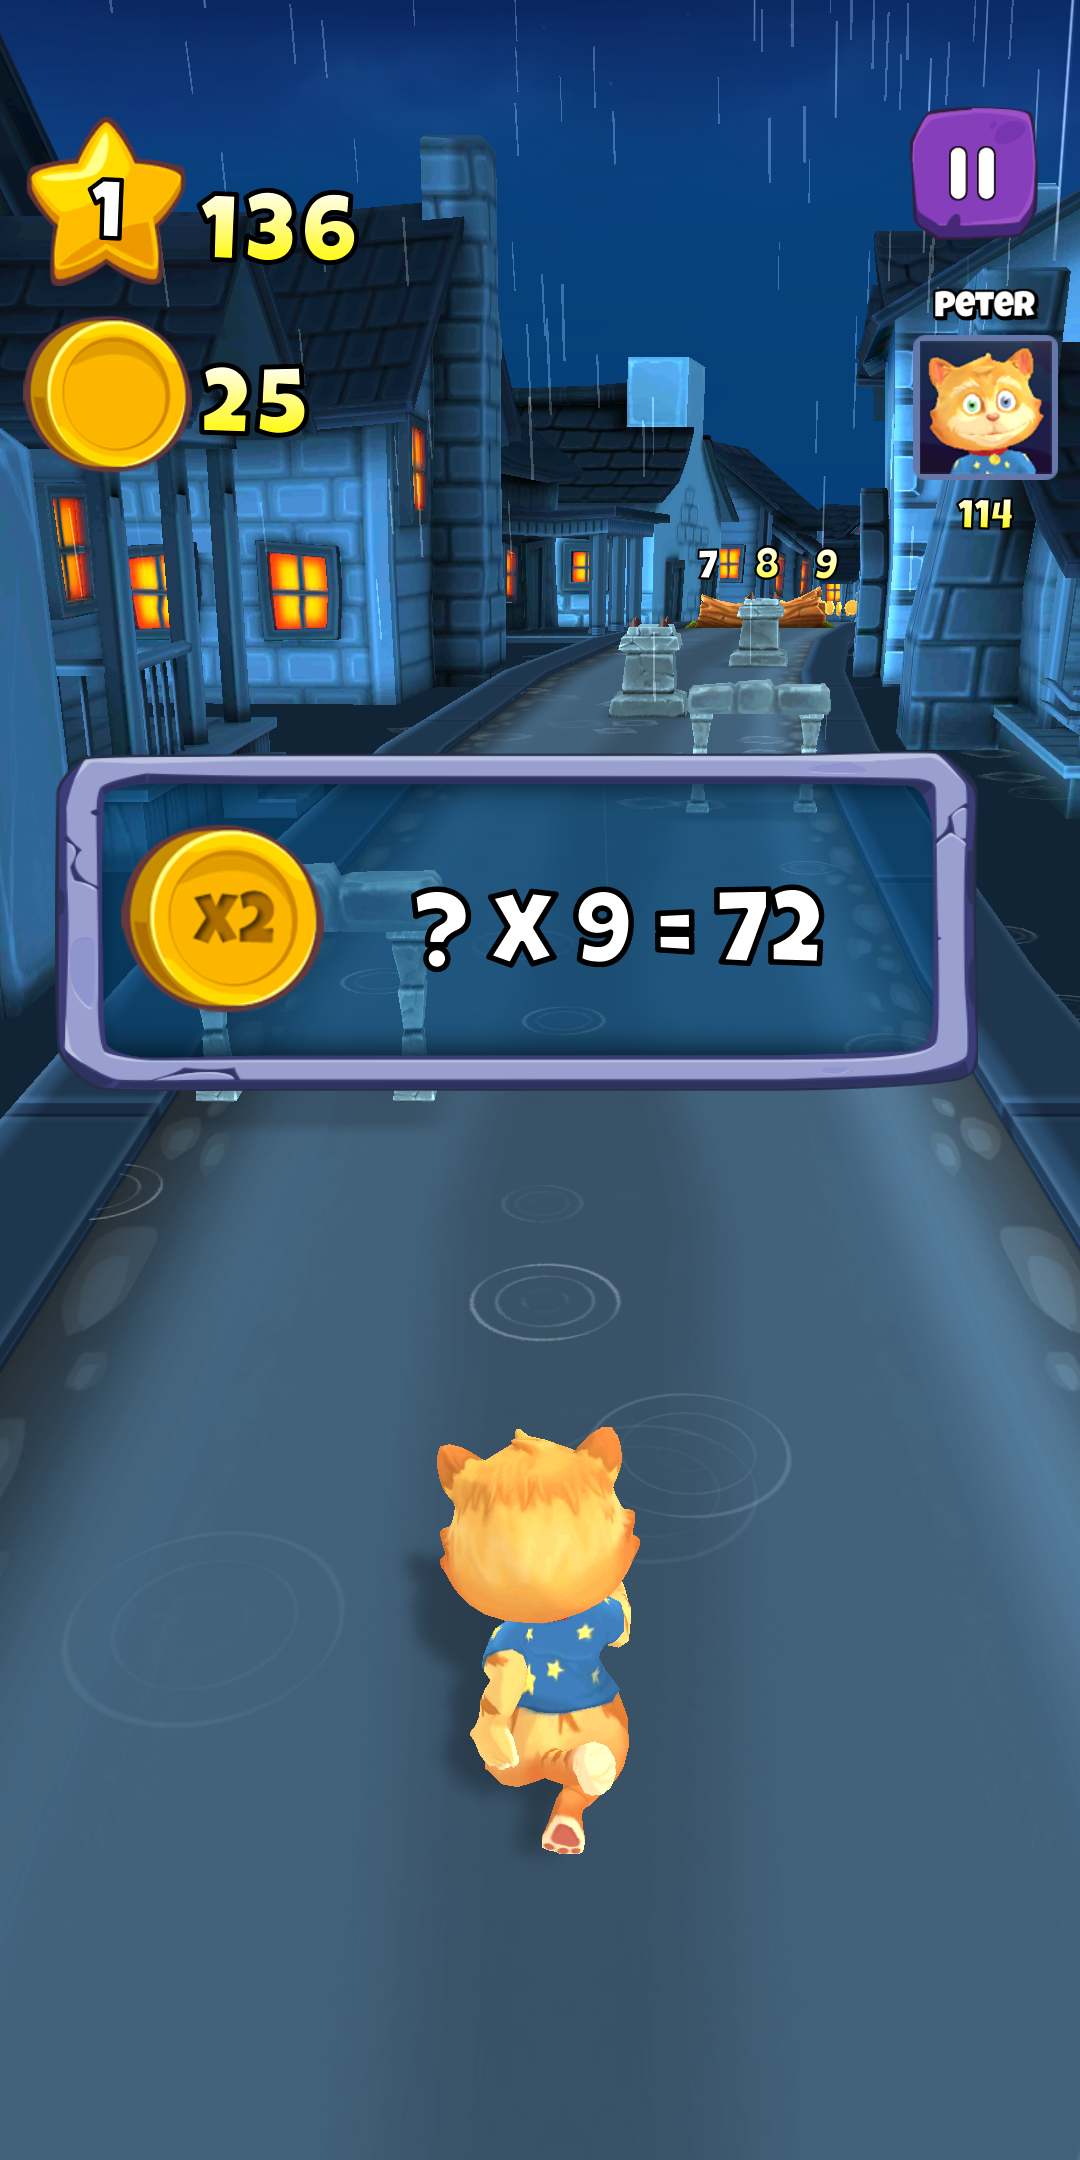
\includegraphics[scale=0.15]{"slike/igre/toonmath2.png"} 
				\caption{Matematički zadatak}
				\label{fig:toonmathmath}
			\end{minipage}
		\end{figure}
		
		 Nažalost, TMR nije tkz. "endless runner" uz to što niti vježbanje matematike nije u glavnom fokusu. Glavni fokus igre je sakupljanje novčića uz pojavljivanje jednog matematičkog zadatka u prosjeku jednom u pola minute. Osim što se ova igra 
		 pokušava nazvati igrom za vježbanje matematike, valja naglasiti da je velika zastupljenost reklama u istoj. 
		 
		 Prednost ove igre u odnosu na igru ovog rada je svakako vizualni izgled i mogućnost napretka u vidu otključavanja drugih karaktera, dok je nedostatak manjak matematičkih zadataka te količina reklama.
		 
	
	\section{Math jumps: Math Games}
	"\textit{Math jumps: Math Games}" (u nastavku MJMG) je vizualno lijepa 2.5D mobilna igrica za vježbanje matematike. Ova igrica osim što je vizualno ugodna, osmišljena je na zanimljiv način. Igrač koji igra igricu predstavljen je kao karakter
	u vagonu koji se vozi po tračnicama. Ovim karakterom ne upravlja se izravno već se njegovo postupanje odvija u skladu s time da li je igrač točno odgovorio na postavljeno matematičko pitanje. Npr. ukoliko igrača ispravno odgovori na zadano matematičko
	pitanje, vagon će poskočiti, odnosno skrenuti kada za tim ima potrebu, suprotno vagon će samo nastaviti voziti ravno i odletiti u provaliju, u tom slučaju igrač gubi život. Igrica je tkz. "endless runner" i moguće je podešavati računske operacije
	koje se mogu pojaviti u zadacima. Ova igra također nudi otključavanje raznih "skinova".
	
	\begin{figure}[H]
		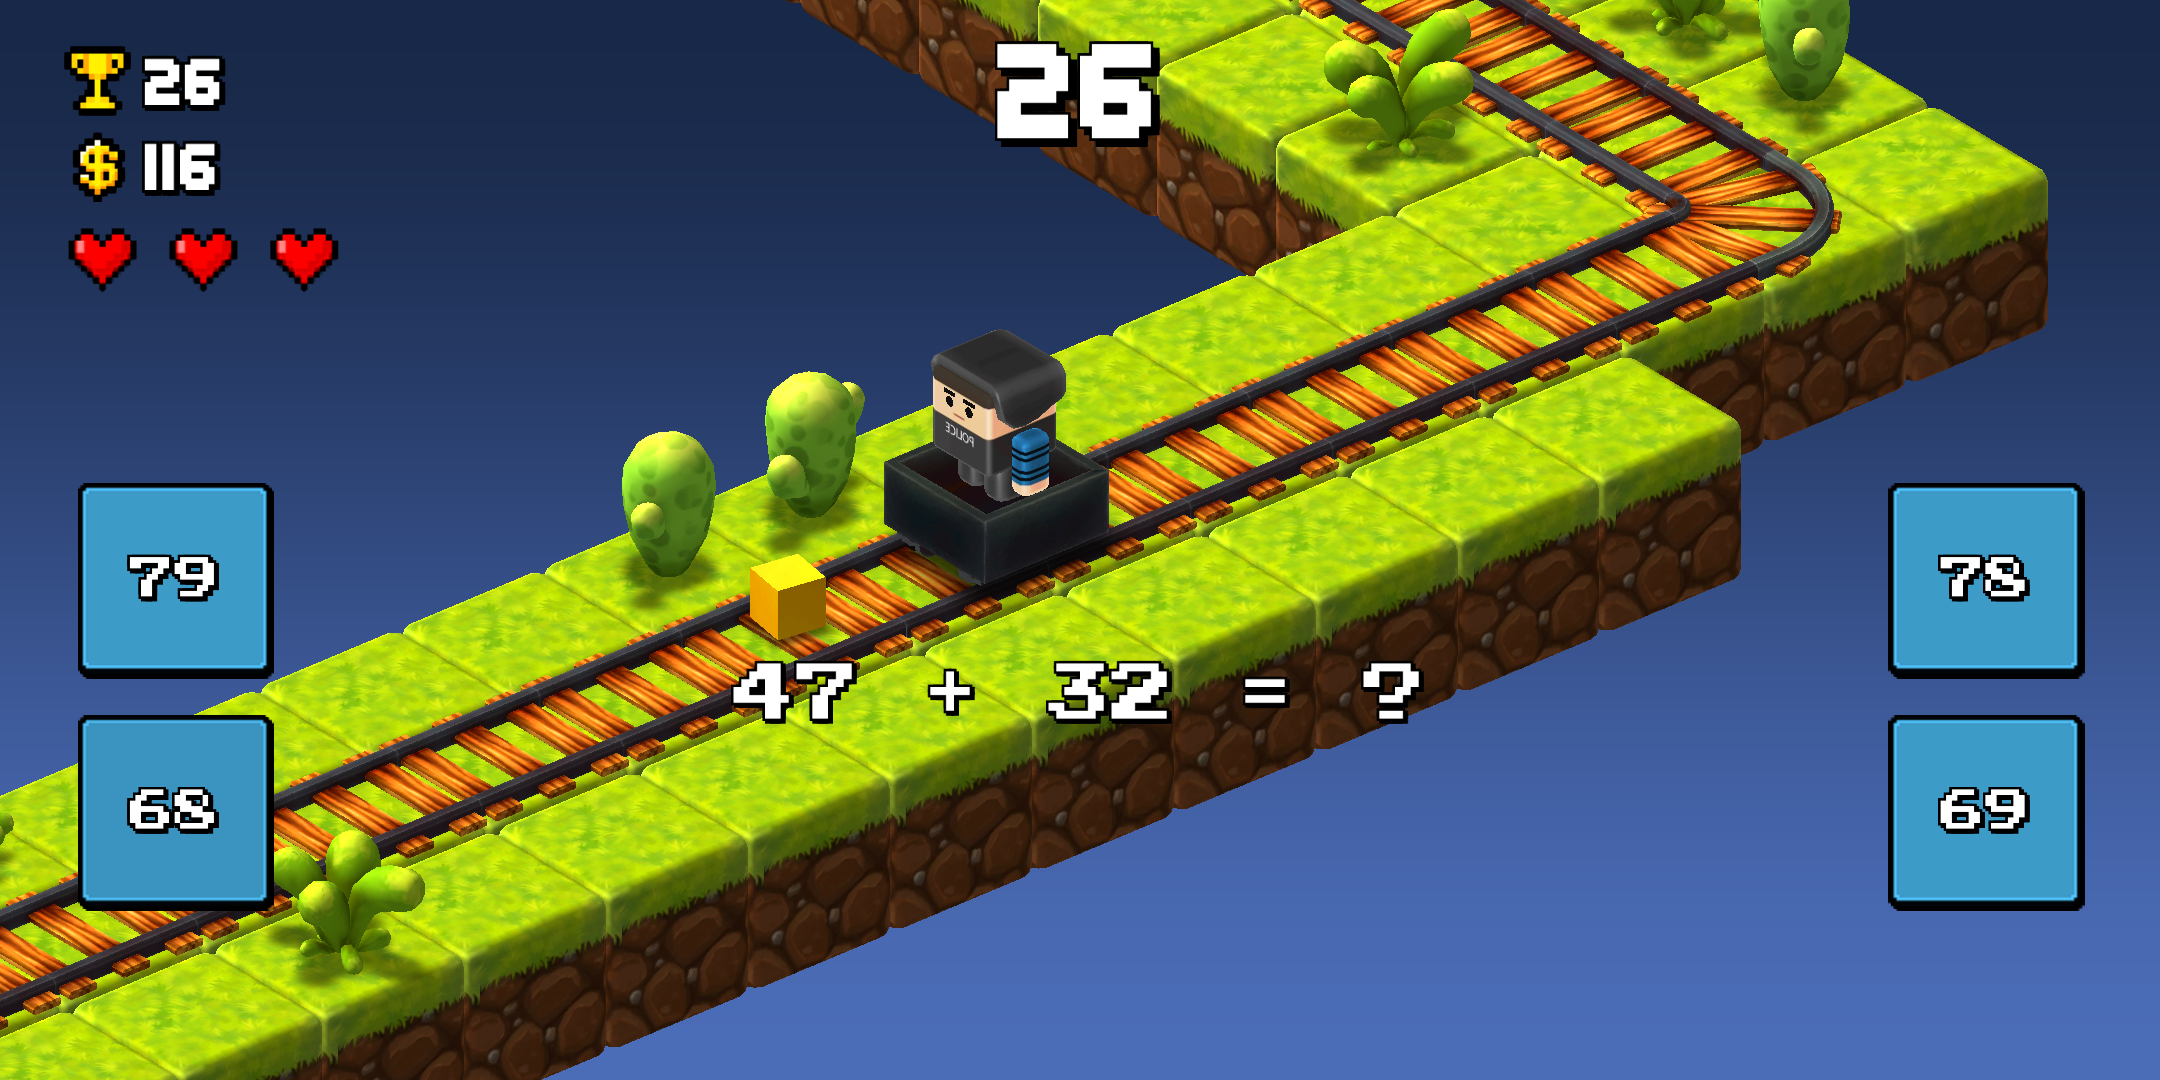
\includegraphics[scale = 0.2]{"slike/igre/mathjumps.png"} 
		\centering
		\caption{Primjer zadatka igre MJMG}
		\label{fig:mjmg}
	\end{figure}
	
	MJMG je u večini aspekata bolja igrica od igrice koja je tema ovog rada no moglo bi se reći da je nedostatak MJMG taj da se sva interakcija odvija putem 4 gumba za odgovore, generalno igrica je običan kviz.
	
	
	\section{Mathematical Run (Math games)}
	"\textit{Mathematical Run (Math games)}" (u nastavku MRMG) je 2D mobila igrica za vježbanje matematike. Igrač koji igra igru upravlja sa malom točkicom koja se može nalaziti u jednoj od tri trake. Na ekranu se prvobitno pojavljuje zadatak, a potom 3
	ponuđena odgovora. Kako bi igrač pokupio ispravan odgovor, treba se pozicionirati u za to odgovarajuću traku. Same kontrole upravljanja su dosta loše, dosta često neresponzivne.
	
			\begin{figure}[!htb]
			\begin{minipage}{0.48\textwidth}
				\centering
				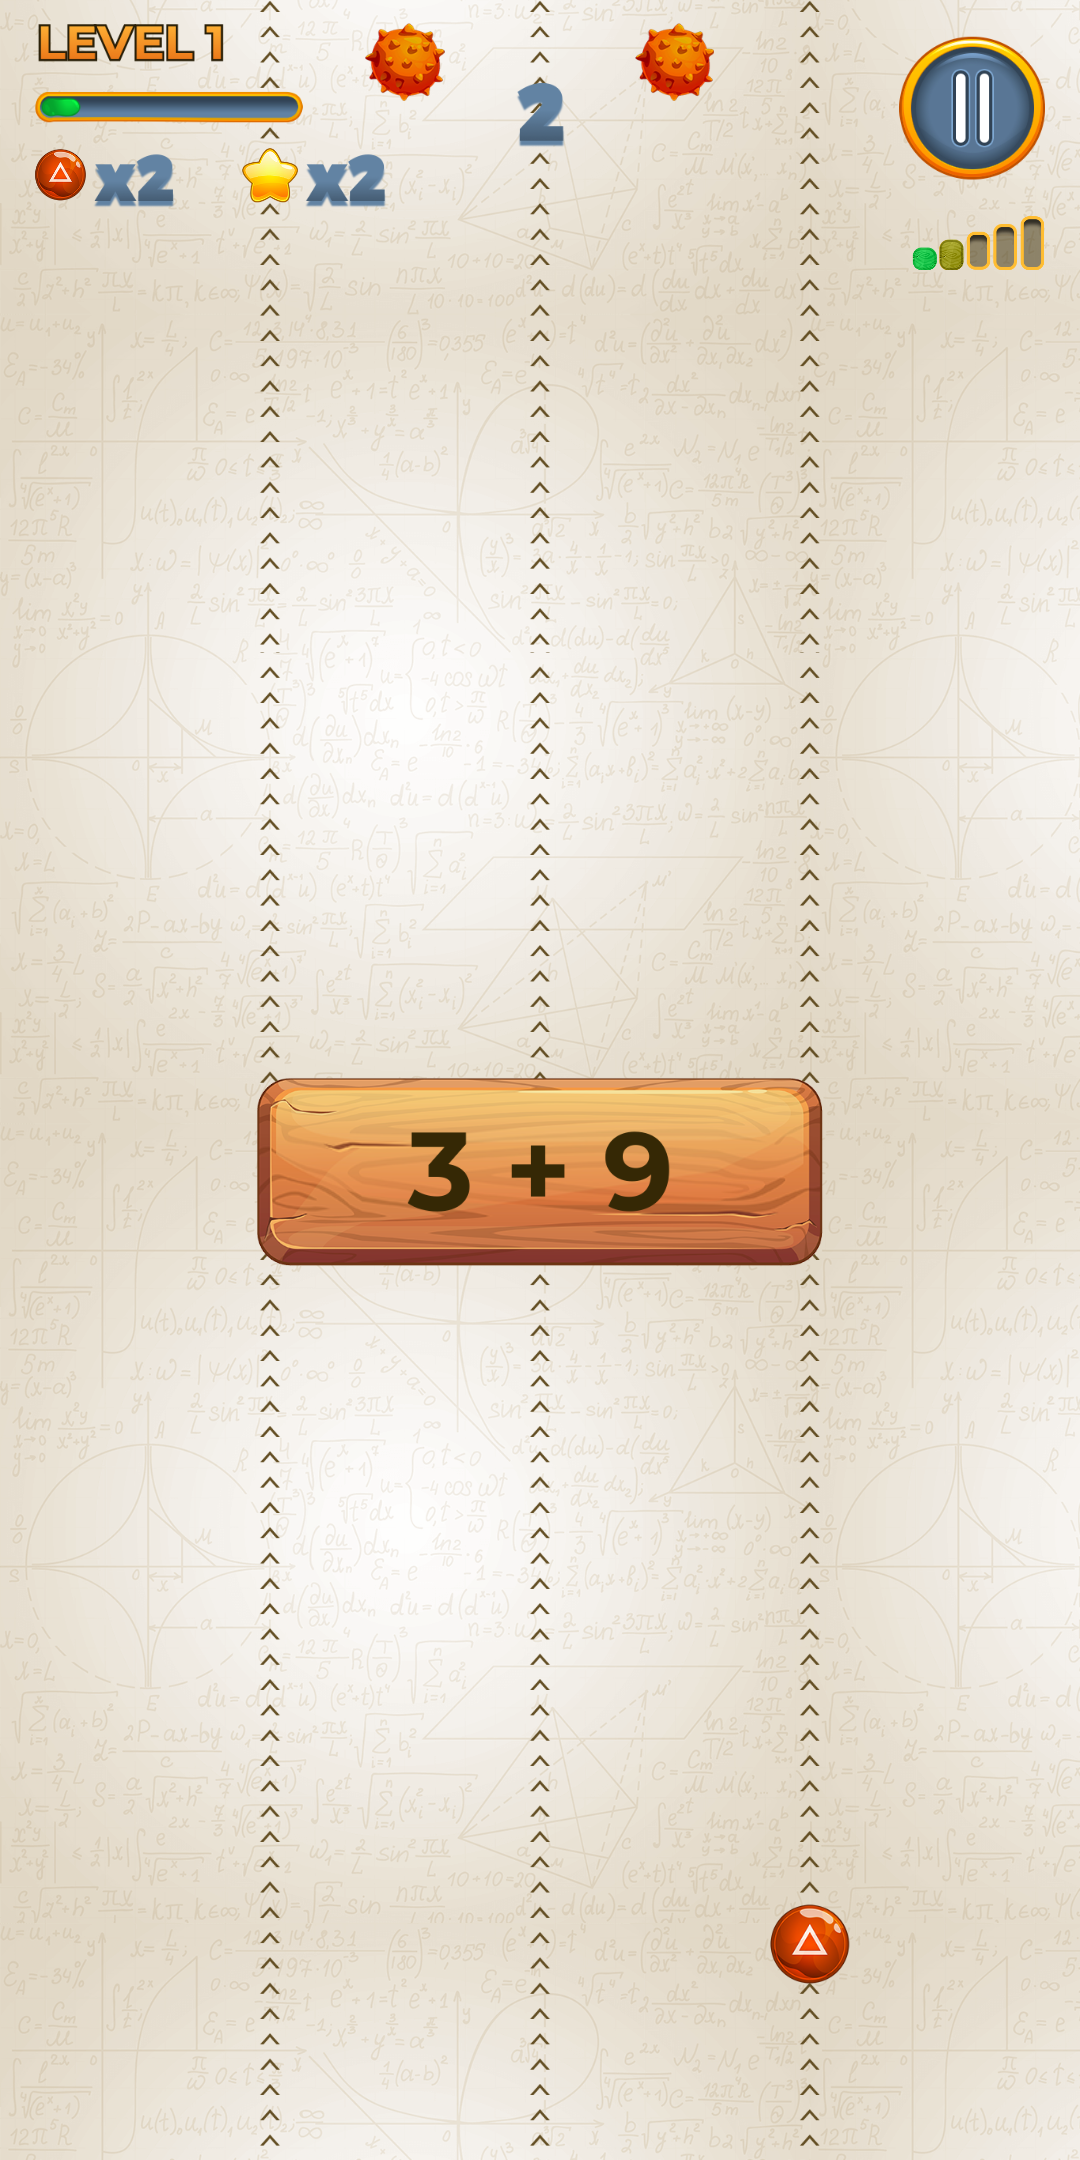
\includegraphics[scale=0.15]{"slike/igre/mathematicalrun1.png"} 
				\caption{Postavljen zadatak}
				\label{fig:zadatak}
			\end{minipage}\hfill
			\begin{minipage}{0.48\textwidth}
				\centering
				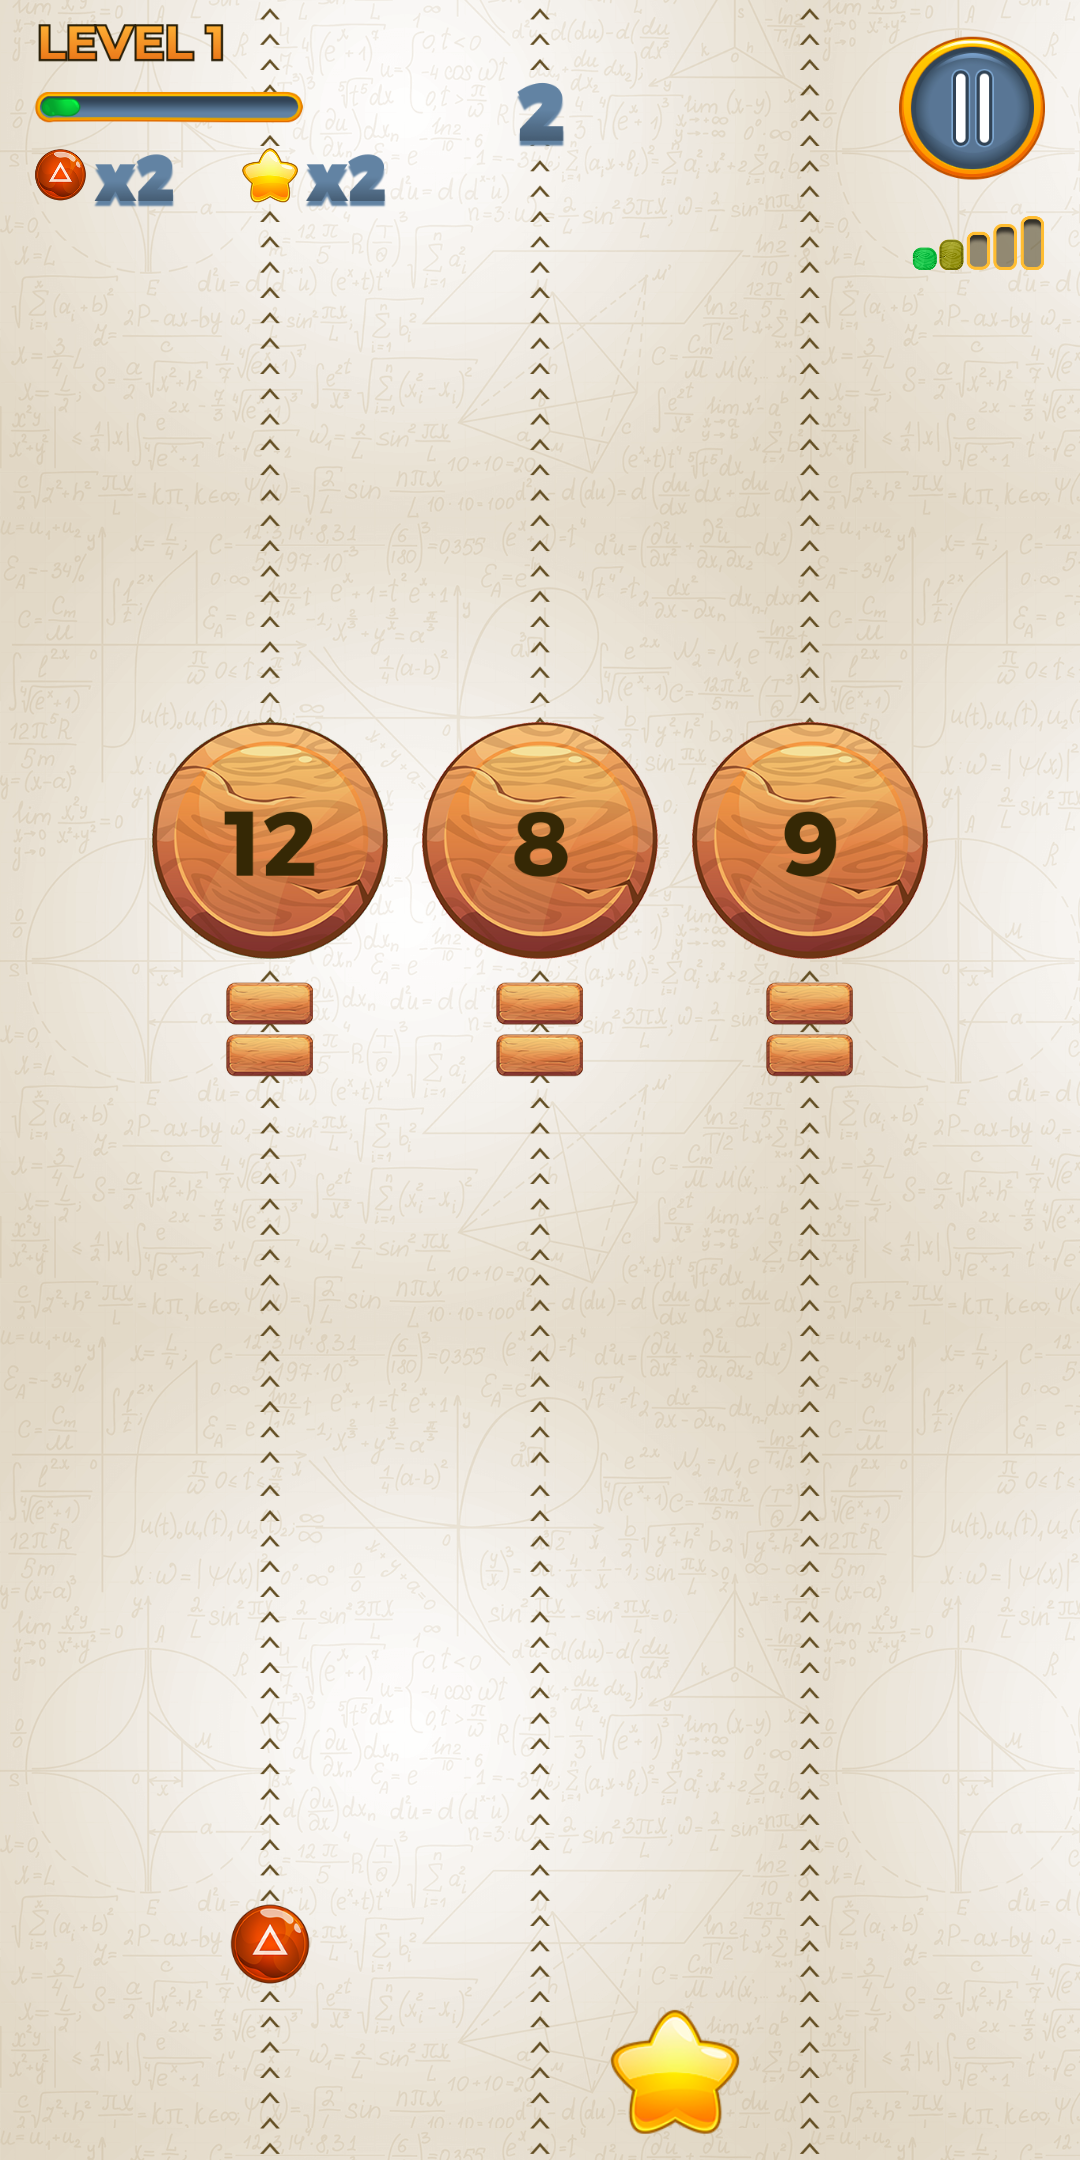
\includegraphics[scale=0.15]{"slike/igre/mathematicalrun2.png"} 
				\caption{Ponuđeni odgovori}
				\label{fig:odgovori}
			\end{minipage}
		\end{figure}

Igrica omogućava odabir tipa zadataka, odnosno zadatak tipa "skupljaj parne brojeve", zadatak tipa "skupljaj manje od x" no ne i sve te zadatke na način da se izmijenuju, već igrač može igrati isključivo jedan zadatak "at the time", tada se na ekranu 
prikazuju samo odgovori, no način igranja je i dalje isti; 3 trake sa neresponzivnim kontrolama. Ova igrica je potencijalno "endless runner". 

\chapter{Korištene tehnologije}
Poglavlje 3

	\section{Java}
	Podpoglavlje 3.1
	
	\section{Node.js}
	Podpoglavlje 3.2

	\section{HTML, CSS}
	Podpoglavlje 3.3

\chapter{Implementacija mobilne igre}

	\section{Pozadina}
	Pozadina je tematski zamišljena kao put iz središta zemlje  do dubokog svemira. Mobilna igra je takozvani endless runner, što znači da se potencijalno može igrati beskonačno,
	odnosno ne postoji način na koji igra završava osim u slučaja da igrač izgubi sve živote, stoga je osim samog efekta "putovanja ka svemiru" potrebno osigurati i beskonačno pomicanje same pozadine.
	
	Pozadina kao takva se u konačnici sastoji od 20ak slika čije spajanje vertikalno daje efekt kontinuiranosti. Dok poznati pokretački strojevi (engl. \textit{game engine}) poput Unity nudi opcije manipulacija
	pozadinom, kao što je beskonačno ponavljajuća pozadina, ta mogućnost u ovakvom razvoju aplikacije nije moguća, već ju je potrebno iskodirati samostalno. 
	Za početak je potrebno učitati slike pozadina kao Bitmap te ih omotati u objekte kako bi im se dala različita svojstva poput x i y koordinata gdje se trenutno nalaze. Takvi objekti pohranjeni su u polje.
	
	Radi jednostavnosti, svaka slika pozadine se  vertikalno i horizontalno skalira na broj piksela koje zaslon mobitela ima; zbog toga, u jednom trenutku na zaslonu se mogu vidjeti maksimalno dvije slike
	pozadine od jednom. Na samom početku igre uzimaju se prva dva objekta pozadine iz polja. Prvi objekt predstavlja donju pozadinu koja će biti prikazana, a drugi gornju pozadinu.  Donju pozadinu potrebno je inicijalizirati
	na lokaciju sa x koordinatom 0 i y koordinatom 0, odnosno želimo da se pokazuje od početka zaslona vertikalno i horizontalno. Drugu sliku inicijaliziramo opet tako da joj damo x koordinatu 0, no y koordinatu postavljamo
	na minus vertikalnu veličinu zaslona. Na svako ponovno osvježavanje igre, pozadina se vertikalno spušta ka dolje čime se stvara efekt putovanja igrača prema gore. Spuštanje pozadine prema dolje implementacijski je 
	ostvareno tako što se svakim osvježavanjem zaslona povećava y koordinata obje slike za određenu vrijednost, ovisno o tome kojom brzinom želimo da "igrač putuje ka svemiru". 
	
	Na sljedećoj slici može se vidjeti način iscrtavanja pozadine na ekranu i izvan njega.
	
	\begin{figure}[H]
			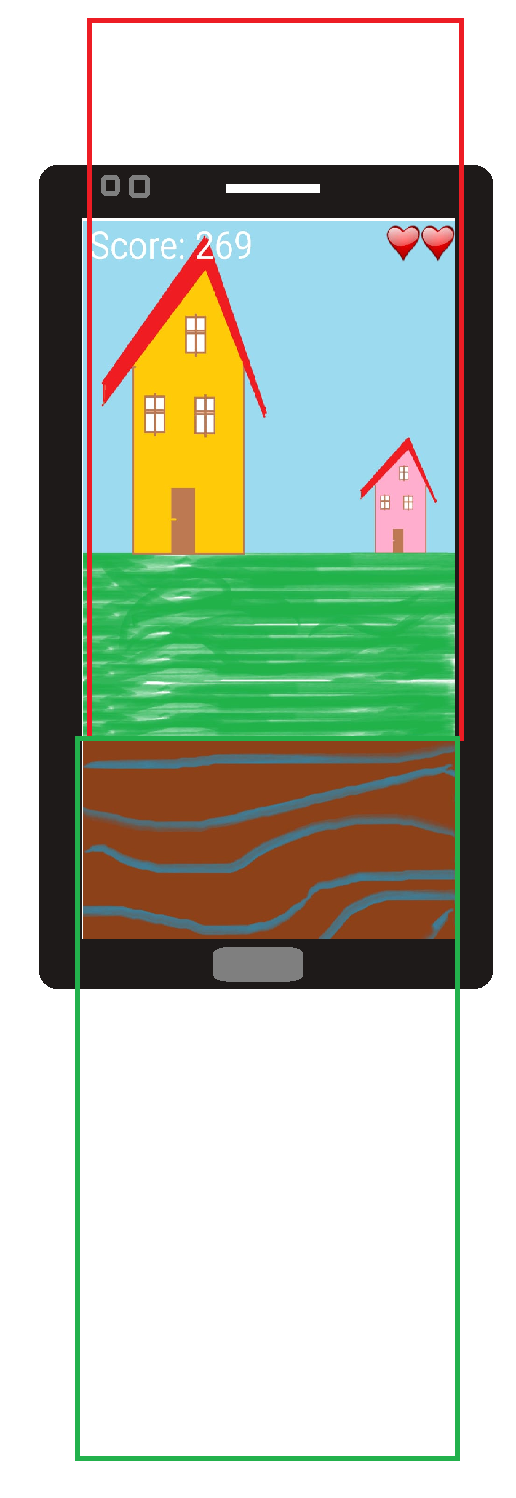
\includegraphics[scale=0.6]{"slike/background.png"} 
			\centering
			\caption{Pomicanje pozadine}
			\label{fig:pomicanjepozadine}
	\end{figure}
		

	
	U trenutku kada y koordinata donje slike izađe izvan ekrana (odnosno kada je vrijednost y osi veća od y dimenzije ekrana) nova donja slika sada je slika koja je bila gore, a novu gornju sliku uzimamo 
	kao sljedeći član polja. 
	Zadnja slika prikazuje svemir pun zvijezdi i nju u polje učitavamo dva puta (dva različita objekta). U trenutku kad smo u igri došli do te slike, tim dvijema slikama se konstanto mijenjaju vrijednosti y osi.
	Odnosno kad donja slika izađe dolje s ekrana, ponovno se postavljaju vrijednosti y osi za obje slike. 
	
	
	Cijeli način implementacije pomicanja pozadine možemo prikazati sljedećim kodom:
	
	\begin{lstlisting}[language = Java , frame = trBL , firstnumber = 1 , escapeinside={(*@}{@*)}]
   private void updateBackground() {
        currentDownBackground.setY(currentDownBackground.getY() + 5);
        currentUpBackground.setY(currentUpBackground.getY() + 5);

        if (currentDownBackground.getY() > screenY) {
            currentDownBackground = currentUpBackground;
            if (currentBackgroundIndex < backgrounds.length - 1)     
                currentUpBackground = backgrounds[++currentBackgroundIndex]; 
            else {
                currentDownBackground = backgrounds[backgrounds.length - 2];
                currentDownBackground.setY(0);
                currentUpBackground = backgrounds[backgrounds.length - 1];
            }
            currentUpBackground.setY(-screenY);
        }
    }
	\end{lstlisting}


	\section{Objekt za skupljanje}
	Slično kao i pozadinu, objekt koji se kontrolira, odnosno objek s kojim se skupljaju padajući objekt učitan je kao kao Bitmap, odnosno više njih, konkretnije kao dva Bitmap objekta omotana sa objektom
	klase "Saw". Za razliku od pozadine koja je putovala prema dolje, objekt s kojim skupljamo padajuće objekte je statičan na ekranu, odnosno ne mijenja svoj položaj na ekranu bez korisničke akcije. Pod kornisničku akciju u 
	ovom slučaju podrazumijeva se dodir ekrana. Koristeći oblikovni obrazac promatrač (engl. \textit{observer}), pri inicijalizaciji igre  subjektu (objektu konkretne klase "View", u ovom slučaju to je "SurfaceView")
	se postavlja konkretna implementacija apstraktnog promatrača "OnTouchListener". Navedeno sučelje sastoji se od jedne funkcije:
	\begin{lstlisting}[language = Java , frame = none , numbers=none, escapeinside={(*@}{@*)}]
		boolean onTouch(View v, MotionEvent event); 
	\end{lstlisting}
	
	Ova funkcija prima dva parametra, "View v" koji je pokazivač na "View" kojem je događaj dodira dostavljen te parametar "MotionEvent event" koji opisuje tip događaja. Primjeri tipova događaja su: 
	"ACTION\_DOWN" koji govori da se dogodio pritisak na zaslonu, "ACTION\_UP" koji govori da je dodir zaslona otpušten, "ACTION\_MOVE" koji govori da se dogodila promjena pozicije između pritiska ("ACTION\_DOWN") i otpuštanja
	("ACTION\_UP") te nekolicina raznih drugih akcija. Navedena funkcija vraća primitivni tip boolean koji u ovom slučaju predstavlja zastavicu koja govori da li je konkretni promatrač "konzumirao događaj do kraja".
	
	U nastavku je prikazan cijeli programski kod potreban za pomicanje objekta za skupljanje. Konkretna implementacija sučelja "OnTouchListener" izvedena je kao anonimni razred, odnosno zbog bolje preglednosti koda 
	koristi se pokrata u vidu lambda izraza, dok "this" predstavlja objekt klase View.

		\begin{lstlisting}[language = Java , frame = trBL , firstnumber = 1 , escapeinside={(*@}{@*)}]
			 this.setOnTouchListener((v, event) -> {
            if (event.getAction() == MotionEvent.ACTION_MOVE 
					|| event.getAction() == MotionEvent.ACTION_DOWN) {
                saw.setX((int) event.getX());
            }
            return true;
        });
		\end{lstlisting}
		
	Na ovom programskom kodu potrebno je uočiti da se kontroliranje našeg objekta može dogoditi doticanjem i pomicanjem prsta na bilo kojem dijelu ekrana, no da sam objekt kojeg kontroliramo neće promijeniti 
	vrijednost svoje x osi, odnosno neće se pomicati vertikalno, već se isključivo mijenja vrijednost položaja na horizontalnoj osi; također je bitno uočiti da za pomicanje objekta nije potrebno stisnuti na objekt
	te ga povući, već je dovoljno stisnuti na određeno mjesto na ekranu te će se objektov položaj na horizonalnoj osi teleportirati na željeno mjesto. Iako je ovo programsko riješenje vjerojatno najjednostavnije, 
	kasnije će se ispostaviti da je ujedno i najbolje. Ukratko, može se dogoditi da objekt kojeg kontroliramo bude okružen s padajućim objektima koji se ne smiju pokupiti i stoga je ova mogućnost "teleportiranja" poželjna.
	
	
	Kao što je već ranije navedeno, objekt za skupljanje koji se kontrolira ne mijenja svoj položaj na ekranu (bez prethodne akcije korisnika) već je potreba učitavanja više slika, odnosno stvaranja više Bitmap 
	objekata nastala u svrhu stvaranja animacije. Animacija se stvara tako što se brzo izmijenjuju slike koje se iscrtavaju na zaslonu. Konkretno, ova animacija sastoji se od dvije slike koje se neprestano izmijenuju.
	Prva slika nastala je jednostavnim crtanjem, dok je druga nastala rotacijom za određeni kut te dodavanjem dodatnih detalja. 
	
	Sljedeće dvije slike prikazuju objekt s kojim skupljamo padajuće objekte, odnosno zajedno prikazuju oštricu koja se rotira velikom brzinom.
	
	
	
		\begin{figure}[!htb]
			\begin{minipage}{0.48\textwidth}
				\centering
				
\includegraphics[scale=0.6]{"slike/saw1.png"} 
				\caption{Originalna slika oštrice}
				\label{fig:saw1}
			\end{minipage}\hfill
			\begin{minipage}{0.48\textwidth}
				\centering
				
\includegraphics[scale=0.6]{"slike/saw2.png"} 
				\caption{Zarotirana originalna slika oštrice sa dodatnim detaljima}
				\label{fig:saw2}
			\end{minipage}
		\end{figure}
	
	\section{Padajući objekti}

\chapter{Baza podataka}
	Baze podataka su organizirane kolekcija podataka koje omogućavaju laki pristup podacima, uređivanje podataka i upravljanje istih. U sklopu ovog projekta koristio se
	SQL tip baze podataka, konkretnije PostgreSQL. PostgreSQL je besplatni, open-source sustav za upravljanje bazom podataka (SUBP) iza kojeg je više od 30 godina aktivnog razvoja.
	
	
	\section{ER dijagram}
		Sljedeća slika prikazuje ER dijagram baze podataka.
		\begin{figure}[H]
			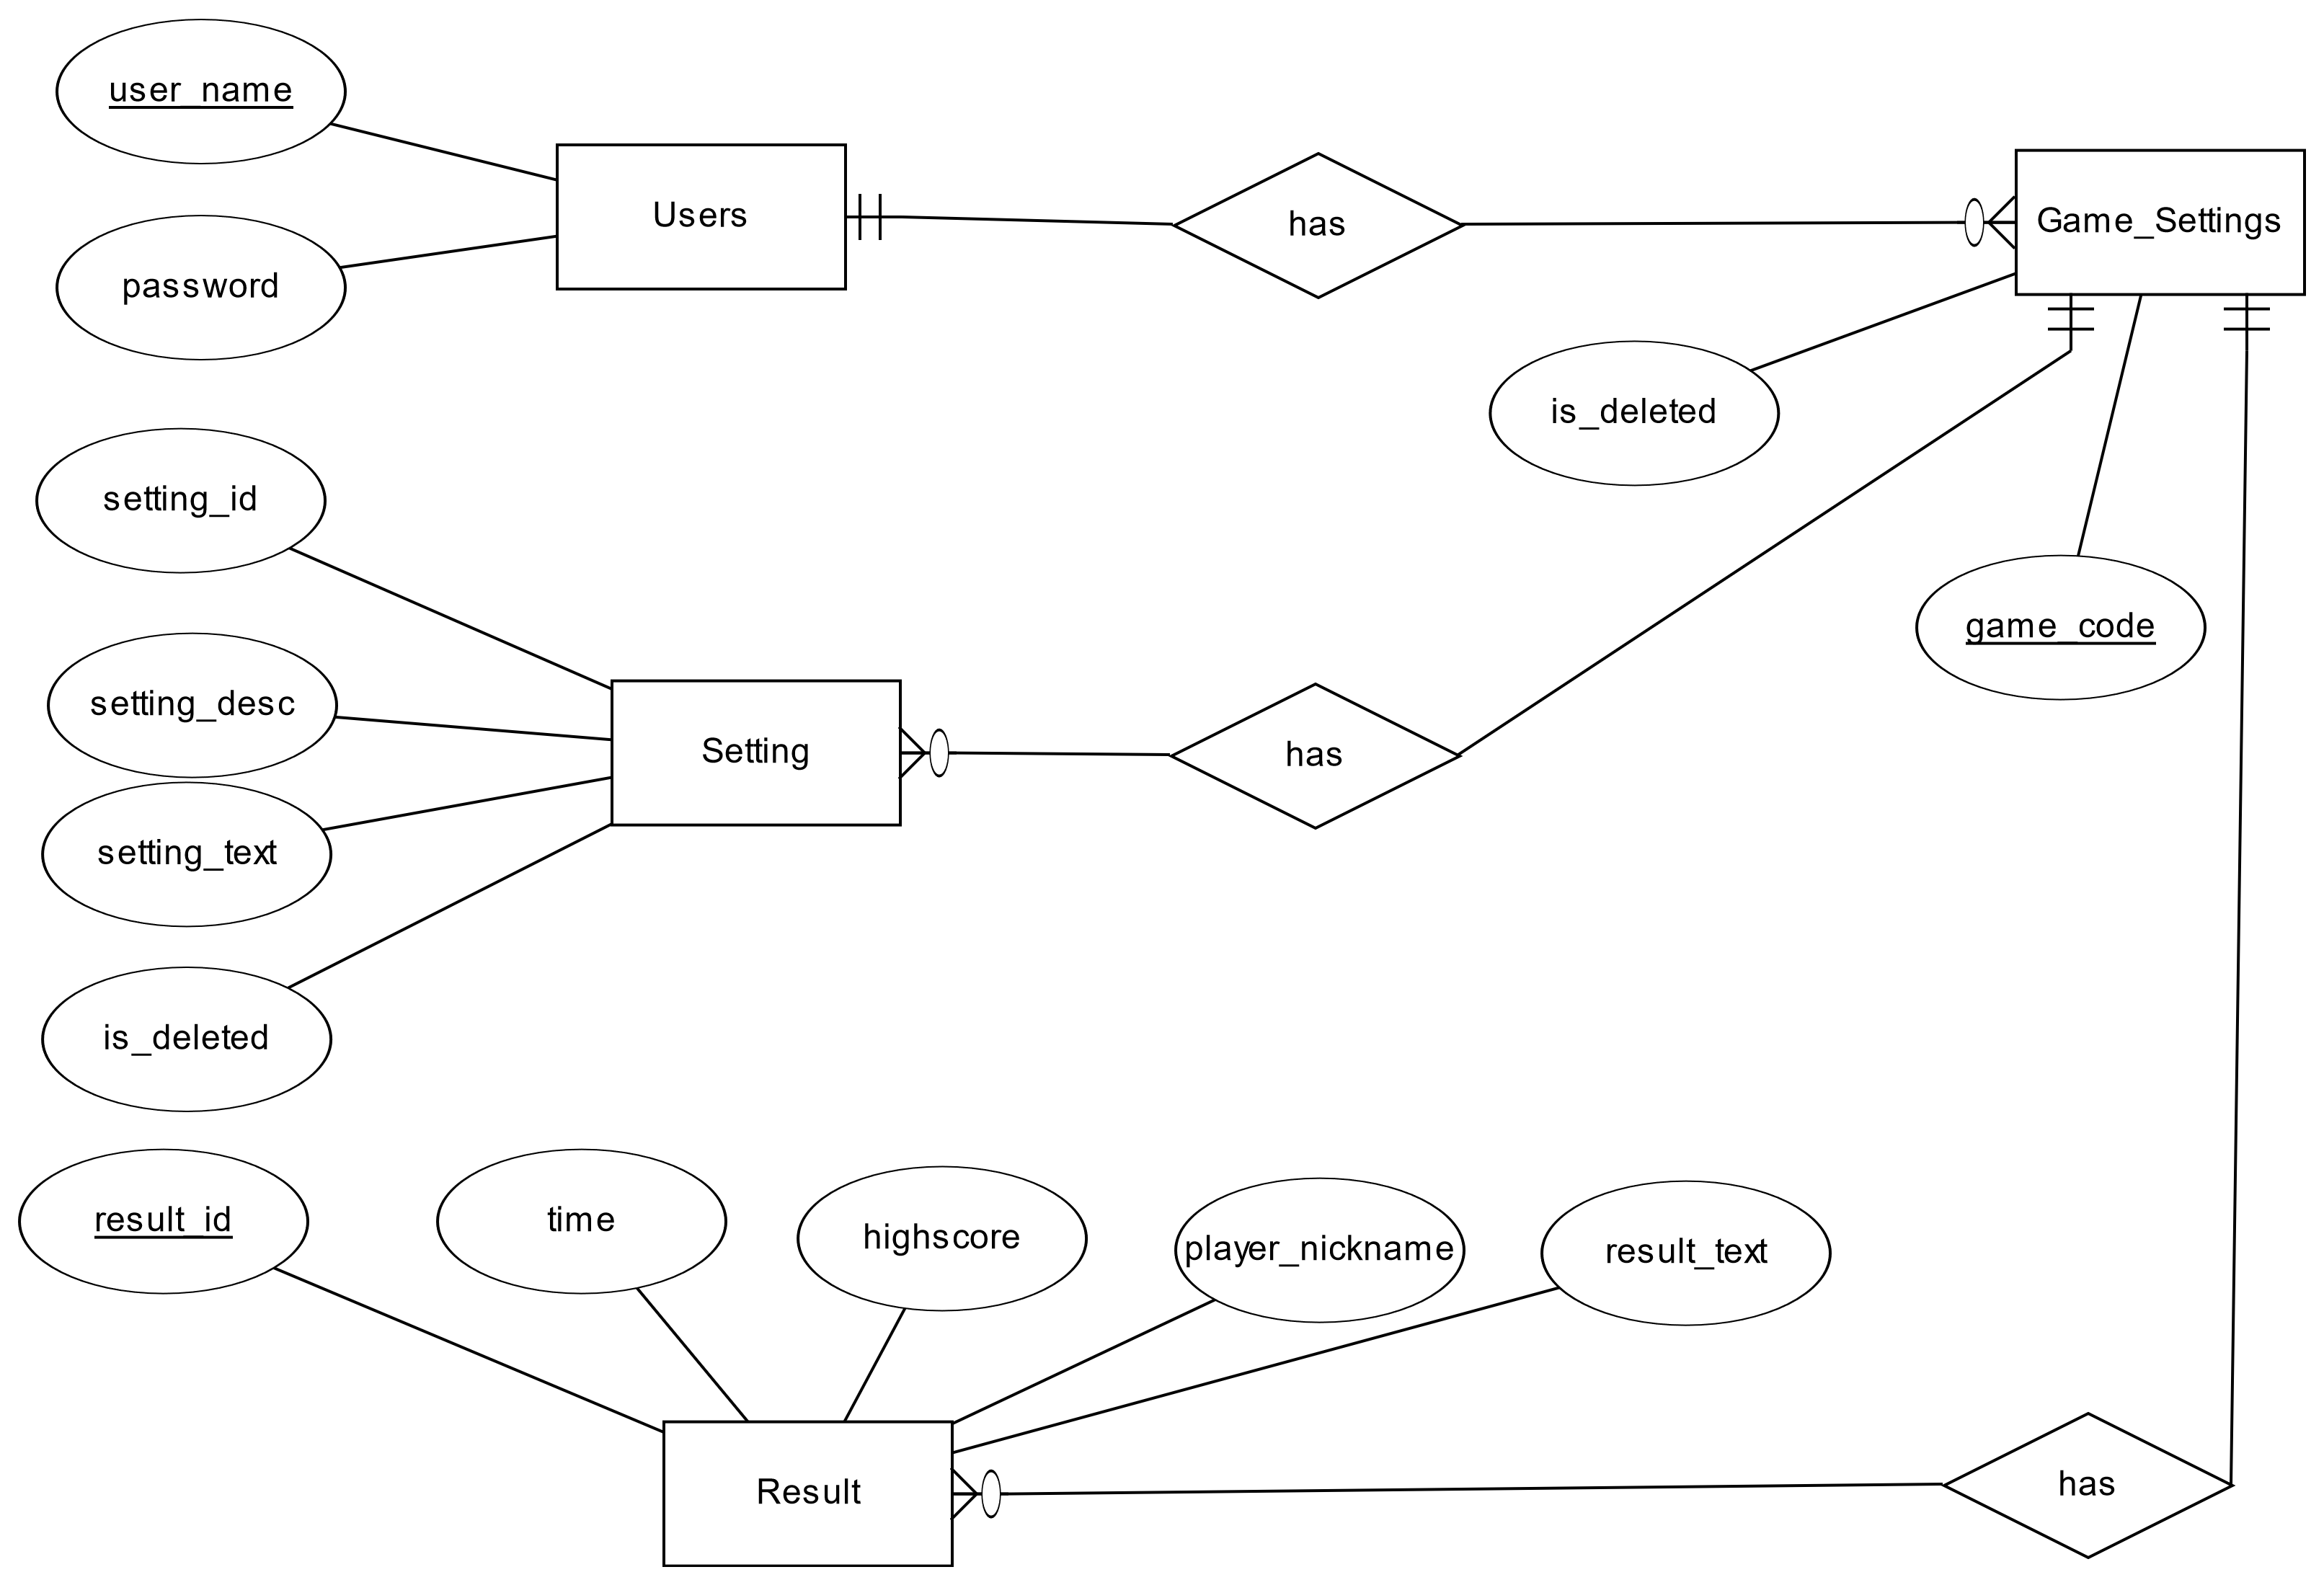
\includegraphics[width=\linewidth]{"slike/ER.png"} 
			\centering
			\caption{ER dijagram baze podataka}
			\label{fig:erdijagram}
		\end{figure}

	
	\section{Opis entiteta i tablica}
			\textbf {Users} \hspace{5mm}
			{Ovaj entitet označava korisnika koji koristi web aplikaciju, odnosno web sučelje za učitelja. Sadrži atribute: user\_ name i password.
			Atribut user\_ name predstavlja korisničko ime korisnika, dok atribut password označava zaporku koja se ne sprema u "plain-textu", već kao 
			rezultat hash funkcije.
			Ovaj entitet u vezi je \textit{One-To-Many} s entitetom Game\_ Settings preko atributa user\_name.}
				
				\begin{longtblr}[
					label=none,
					entry=none
					]{
						width = \textwidth,
						colspec={|X[6,l]|X[6, l]|X[20, l]|}, 
						rowhead = 1,
					} %definicija širine tablice, širine stupaca, poravnanje i broja redaka naslova tablice
					\hline \multicolumn{3}{|c|}{\textbf{Users}}	 \\ \hline[3pt]
					\SetCell{LightGreen}user\_name & VARCHAR	&  	jedinstveni naziv korisnika  	\\ \hline
					password	& VARCHAR &  rezultat hash funkcije nad zaporkom 	\\ \hline 
				\end{longtblr}



			\textbf {Game\_ Settings} \hspace{5mm}
			{Ovaj entitet označava jedan "game room". Sadrži atribute: game\_ code i is\_ deleted.
			Ovaj entitet u vezi je \textit{Many-To-One} s entitetom Users preko atributa user\_ name, u vezi \textit{One-To-Many} s
			entitetom Setting preko atributa game\_ code te u vezi \textit{One-To-Many} s entitetom Result preko atributa game\_ code.}
				
				\begin{longtblr}[
					label=none,
					entry=none
					]{
						width = \textwidth,
						colspec={|X[6,l]|X[6, l]|X[20, l]|}, 
						rowhead = 1,
					} 
					\hline \multicolumn{3}{|c|}{\textbf{Game\_ Settings}}	 \\ \hline[3pt]
					\SetCell{LightGreen}game\_ code & INT	&  	jedinstveni idenfitikator game\_ settings   	\\ \hline
					is\_ deleted & INT & zastavica koja govori jesu li "game room" obrisan \\ \hline
					\SetCell{LightBlue}user\_ name & VARCHAR & oznaka korisnika kojem "game room" pripada \\ \hline
				\end{longtblr}


			\textbf {Setting} \hspace{5mm}
			{Ovaj entitet označava jedanu postavku. Sadrži atribute: setting\_ id, setting\_ desc, setting\_ text i is\_ deleted.
			Ovaj entitet u vezi je \textit{Many-To-One} s entitetom Game\_ Settings preko atributa game\_ code.}
				
				\begin{longtblr}[
					label=none,
					entry=none
					]{
						width = \textwidth,
						colspec={|X[6,l]|X[6, l]|X[20, l]|}, 
						rowhead = 1,
					} 
					\hline \multicolumn{3}{|c|}{\textbf{Setting}}	 \\ \hline[3pt]
					\SetCell{LightGreen}setting\_ id & INT	&  	jedinstveni idenfitikator za Setting  	\\ \hline
					setting\_desc & VARCHAR & tekst koji opisuje cilj zadatka \\ \hline
					setting\_text & VARCHAR & postavka formatirana tako da bude razumljiva mobilnoj igri \\ \hline
					is\_ deleted & INT & zastavica koja govori je li postavka obrisana \\ \hline
					\SetCell{LightBlue}game\_code & INT & oznaka Game\_Settings kojem Setting pripada \\ \hline
					
				\end{longtblr}
				
			
			\textbf {Result} \hspace{5mm}
			{Ovaj entitet označava jedan rezultat igranja igre na mobitelu uz preuzete postavke.
			Sadrži atribute: result\_ id, time, highscore, player\_ nickname te result\_ text.
			Ovaj entitet u vezi je \textit{Many-To-One} s entitetom Game\_ Settings preko atributa game\_ code.}
				
				\begin{longtblr}[
					label=none,
					entry=none
					]{
						width = \textwidth,
						colspec={|X[6,l]|X[6, l]|X[20, l]|}, 
						rowhead = 1,
					} 
					\hline \multicolumn{3}{|c|}{\textbf{Result}}	 \\ \hline[3pt]
					\SetCell{LightGreen}result\_ id & INT	&  	jedinstveni idenfitikator za Result  	\\ \hline
					time & VARCHAR & vrijeme pohrane rezultata u bazu podatka \\ \hline
					highscore & VARCHAR & ostvareni rezultat na igri  \\ \hline
					player\_ nickname & VARCHAR & nadimak igrača  \\ \hline
					result\_text & VARCHAR & JSON polje s događajima igre  \\ \hline
					\SetCell{LightBlue}game\_code & INT & oznaka Game\_Settings kojem Result pripada \\ \hline
					
				\end{longtblr}

	\newpage
	\section{Relacijski dijagram}
		Sljedeća slika prikazuje relacijski dijagram baze podataka.
		\begin{figure}[H]
			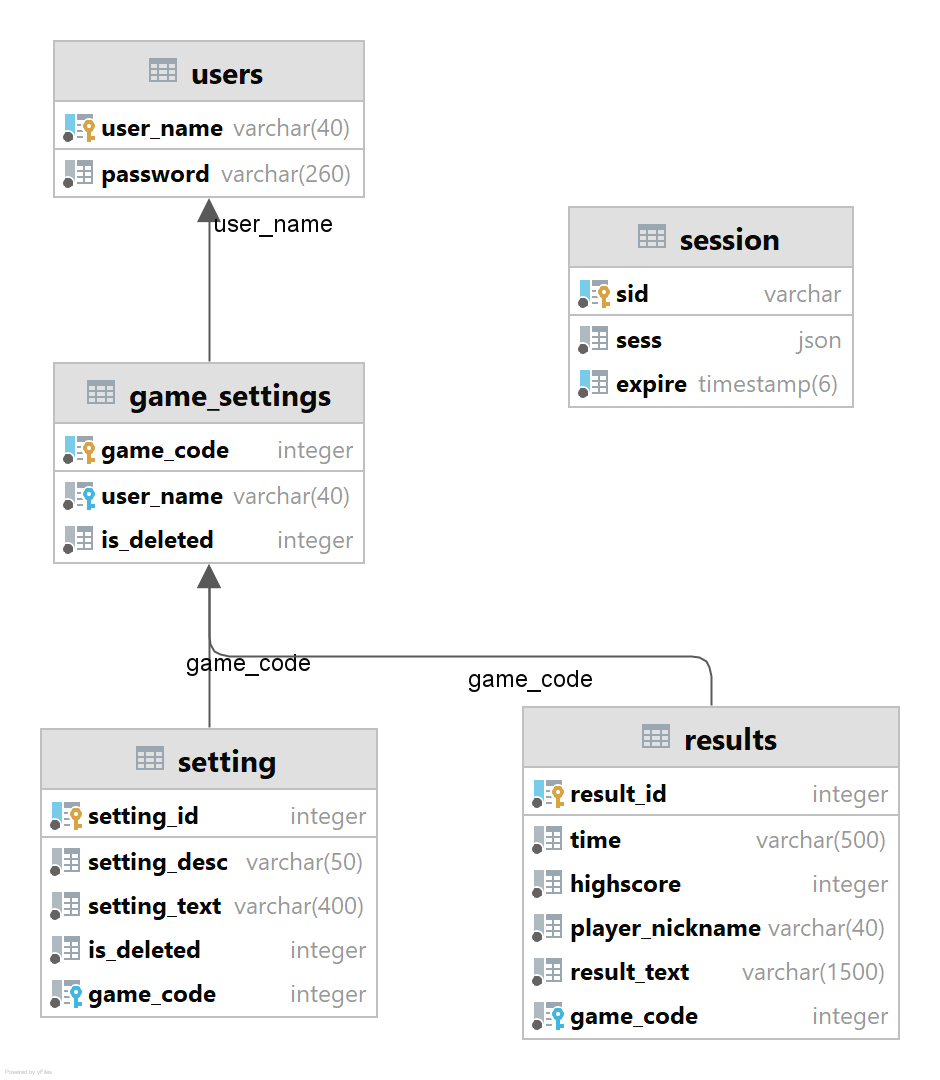
\includegraphics[width=\linewidth]{"slike/REL.png"} 
			\centering
			\caption{Relacijska shema baze podataka}
			\label{fig:relshema}
		\end{figure}


\chapter{Naslov 4}
Poglavlje 4

\bibliography{literatura}
\bibliographystyle{fer}

\begin{sazetak}
Sažetak na hrvatskom jeziku.

\kljucnerijeci{Ključne riječi, odvojene zarezima.}
\end{sazetak}

% TODO: Navedite naslov na engleskom jeziku.
\engtitle{Mobile game for practicing math}
\begin{abstract}
Abstract.

\keywords{Keywords.}
\end{abstract}

\end{document}
